\documentclass[numerate]{cheatsheet}
\usepackage{bm}
\usepackage{textcomp, mathcomp}
\usepackage{empheq}
\usepackage{pbox}
\usepackage{booktabs}

\doctitle{Physik Zusammenfassung}
\author{Noa Sendlhofer, Christian Leser \\\& Gian Maria Ernst \\ nsendlhofer, cleser \& ernstg \\ \vspace*{-0.2em}}

% Noch hinzufügen:
% Mechanische Arbeit: \int\limits_{t_1}^{t_2} P(t) dt
% Additionstheoreme $\cos(\alpha) + \cos(\beta) = 2 cos(\frac{\alpha + \beta}{2}) cos(\frac{\alpha - \beta}{2})$

\begin{document}
\section{Elektrizitätslehre}
    \subsection{Ladung Q \hfill $[C]$}
    \begin{itemize}
        \item Elementarladung: $q_{Elektron} = e = - 1.602 \cdot 10^{-19}C$
    \end{itemize}

    Coulomb-Kraft: 

    \begin{minipage}{0.53\linewidth}
        \begin{footnotesize}
            \begin{center}
                \mathbox{
                    \vec{F_C}=\frac{1}{4\pi\varepsilon_0}\cdot \frac{q_1 \cdot q_2}
                    {r^2}\cdot \vec{e_r}            }
            \end{center}
        \end{footnotesize}
    \end{minipage}
    \begin{minipage}{0.46\linewidth}
        \begin{scriptsize}
            \begin{center}
                \begin{align*}
                    \varepsilon_0 &= 8,854\cdot10^{-12}
                    \\q_{1/2} &= \text{Punktladungen}
                    \\r &= \text{Abstand zw. Punktladungen}
                    \\\vec{e_r} &= \text{Einheitsvektor}
                \end{align*}
            \end{center}
        \end{scriptsize}
    \end{minipage}
    \vspace{1mm}



    \begin{itemize}
        \item Ladungen mit gleichem Vorzeichen stossen sich ab.
        \\$F_C<0 \rightarrow \text{abstossend}$,
        $F_C>0 \rightarrow \text{anziehend}$
        \item Ladungen leitender Körper stets an Oberfläche.\\
        $\rightarrow$ Inneres: Ladungs und Feldfrei
    \end{itemize}

    \subsubsection{Ladungsdichte}
        \begin{tabular}{c c c}
            Liniendichte $\lambda$ & Oberflächendichte $\sigma$ & Volumendichte $\rho$ \\
            $\lambda = \frac{Q}{l} \left[\frac{C}{m}\right]$ & $\sigma = \frac{Q}{A} \left[\frac{C}{m^2}\right]$ & $\rho = \frac{Q}{V} \left[\frac{C}{m^3}\right]$
        \end{tabular}


    \subsection{Strom I \hfill $[A]$}
    Strom A:

    \vspace{-1mm}\begin{minipage}{0.4\linewidth}
        \begin{footnotesize}
            \begin{center}
                \mathbox{
                    I = \frac{dQ}{dt} \left[\frac{C}{s}\right]
                }
                
            \end{center}
        \end{footnotesize}
    \end{minipage}
    $\longleftrightarrow$
    \begin{minipage}{0.4\linewidth}
        \begin{footnotesize}
            \begin{center}
                \mathbox{
                    Q = \int\limits_{\Delta t} I dt
                }
            \end{center}
        \end{footnotesize}
    \end{minipage}
    \vspace{1mm}

    Stromdichte j:

    \vspace{-1mm}\begin{minipage}{0.25\linewidth}
        \begin{footnotesize}
            \begin{center}
                \mathbox{
                    j = \frac{I}{A} \left[\frac{A}{m^2}\right]
                }
                
            \end{center}
        \end{footnotesize}
    \end{minipage}
    $\longleftrightarrow$
    \begin{minipage}{0.55\linewidth}
        \begin{footnotesize}
            \begin{center}
                \mathbox{
                    I = \iint\limits_{A} j dA \overset{(\text{$I$ gleichm. auf $A$})}{=} j \cdot A
                }
            \end{center}
        \end{footnotesize}
    \end{minipage}
    \vspace{1mm}

    \subsubsection{Stromdichte}
        \begin{tabular}{c c c}
            & Flächendichte $j$ &\\
            & $j = \frac{I}{A} \left[\frac{C}{s \cdot m^2}\right]$ &
        \end{tabular}


    \subsection{Elektrischer Widerstand R \hfill $[\Omega]$}
    Widerstand: \mathbox{R = \frac{U}{I}, I \sim U}

    \begin{tabular}{c c}
        Ohmsche Leiter & nicht-ohmsche Leiter \\
        $I = \frac{U}{R}$ & $R_{\text{diff}} = \frac{dU}{dI}$\\
        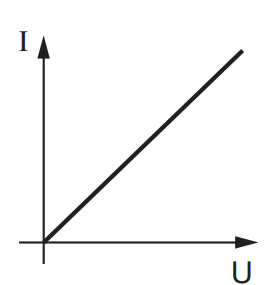
\includegraphics[width = 30mm]{src/images/plot_ohmscher_leiter.png} & 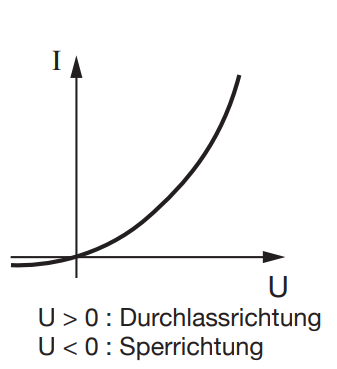
\includegraphics[width = 30mm]{src/images/plot_nicht-ohmscher_leiter.png}
    \end{tabular}
    \vfill

    \subsubsection{Spezifischer Widerstand}
        nach Grösse:

        \vspace{-1mm}
        \begin{minipage}{0.49\linewidth}
            \begin{footnotesize}
                \begin{center}
                    \mathbox{
                        R = \rho \frac{l}{A}
                    }
                \end{center}
            \end{footnotesize}
        \end{minipage}
        \begin{minipage}{0.5\linewidth}
            \begin{scriptsize}
                \begin{center}
                    \begin{align*}
                        l &= \text{Leiterlänge}
                        \\A &= \text{Leiterquerschnitt} 
                        \\\rho &= \text{spezifischer Widerstand}
                        \\  K &= \frac{1}{\rho} = \text{Spezifische Leitfähigkeit}
                    \end{align*}
                \end{center}
            \end{scriptsize}
        \end{minipage}
        \vspace{1mm}

        nach Temperatur:

        \vspace{-1mm}
        \begin{minipage}{0.49\linewidth}
            \begin{footnotesize}
                \begin{center}
                    \mathbox{
                        \rho(T) = \rho_0 (1 + \alpha(T - T_0))
                    }
                \end{center}
            \end{footnotesize}
        \end{minipage}
        \begin{minipage}{0.5\linewidth}
            \begin{scriptsize}
                \begin{center}
                    \begin{align*}
                        \rho_0 &= \text{spezifischer Widerstand bei } T_0
                        \\T_0 &= \text{Bezugstemperatur}
                        \\\alpha &= \frac{1}{K} =\text{Temperaturkoeffizient}
                    \end{align*}
                \end{center}
            \end{scriptsize}
        \end{minipage}
        \vspace{1mm}
    \subsection{Elektrische Kapazität C \hfill $[F]$}
    \begin{minipage}{0.49\linewidth}
        \begin{center}
            Im Vakuum:
            \mathbox{C_0 = \frac{Q}{U} = \varepsilon_0 \frac{A}{l}}
        \end{center}
    \end{minipage}
    \begin{minipage}{0.49\linewidth}
        \begin{center}
            Materie (Dielektrikum mit $\varepsilon_m$):
            \begin{empheq}[box=\fbox]{align*}
                C_m &= \varepsilon_m C_0\\
                U_m &= \frac{U_0}{\varepsilon_m}\\
                \varepsilon_m &= \frac{\overrightarrow{E}_0}{\overrightarrow{E}_m}
            \end{empheq}
        \end{center}
    \end{minipage}

    \begin{minipage}{0.49\linewidth}
        \begin{center}
            Ladestrom Kondensator:
            \begin{empheq}[box=\fbox]{align*}
                I(t) &= I_0 \cdot e^{\left(-\frac{t}{R \cdot C}\right)}\\
                I(0) &= I_0 = \frac{U}{R_{\text{tot}}}\\
                I(\infty) &= 0
            \end{empheq}
        \end{center}
    \end{minipage}
    \begin{minipage}{0.49\linewidth}
        \begin{center}
            \begin{flushleft}
                \begin{scriptsize}
                    Einschieben von Dielektrika in einen Plattenkondensator: \\
                    Die Energieverteilung verändert sich bis ein Gleichgewichtszustand erreicht ist:
                \end{scriptsize}  
            \end{flushleft}
            \begin{empheq}[box=\fbox]{align*}
                0 &= dW_{\text{tot}}\\
                 &\scriptstyle= dW_{\text{Feld}} - dW_{\text{Batt}} + dW_{\text{Diel}}
            \end{empheq}
        \end{center}
    \end{minipage}
    \subsection{Kirchhoffsche Regeln}
    \subsubsection{Knotenregel}
        \vspace{-1mm}
        \begin{minipage}{0.49\linewidth}
            \begin{footnotesize}
                \begin{center}
                    \vspace{2mm}
                    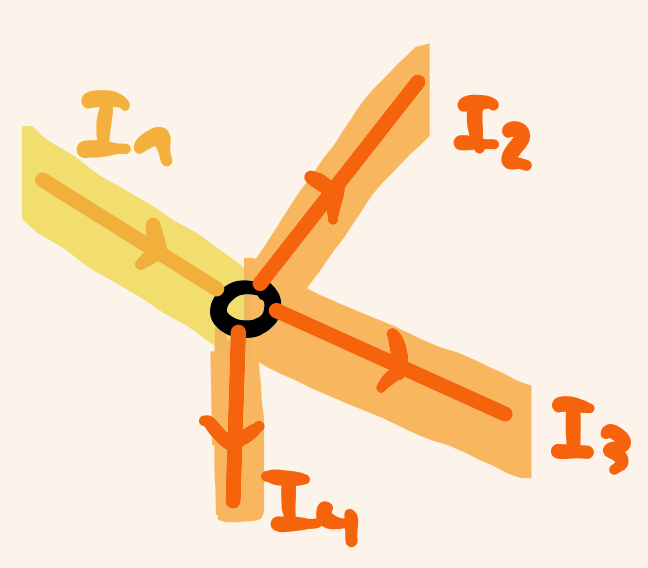
\includegraphics[width = 20mm]{src/images/knotenregel.png}
                \end{center}
            \end{footnotesize}
        \end{minipage}
        \begin{minipage}{0.5\linewidth}
            \begin{scriptsize}
                \begin{center}
                    \begin{align*}
                        \text{Widerstände:} \; &\sum\limits_k I_k = 0\\
                        \text{Kondensatoren:} \; &\sum\limits_k Q_k = 0
                    \end{align*}
                    \colorbox{Goldenrod}{$\sum I_\text{zufliessend}$} $=$ \colorbox{Apricot}{$\sum I_\text{abfliessend}$} 
                \end{center}
            \end{scriptsize}
        \end{minipage}
        \vspace{1mm}

    \subsubsection{Maschenregel}
        \vspace{-1mm}
        \begin{minipage}{0.49\linewidth}
            \begin{footnotesize}
                \begin{center}
                    \vspace{2mm}
                    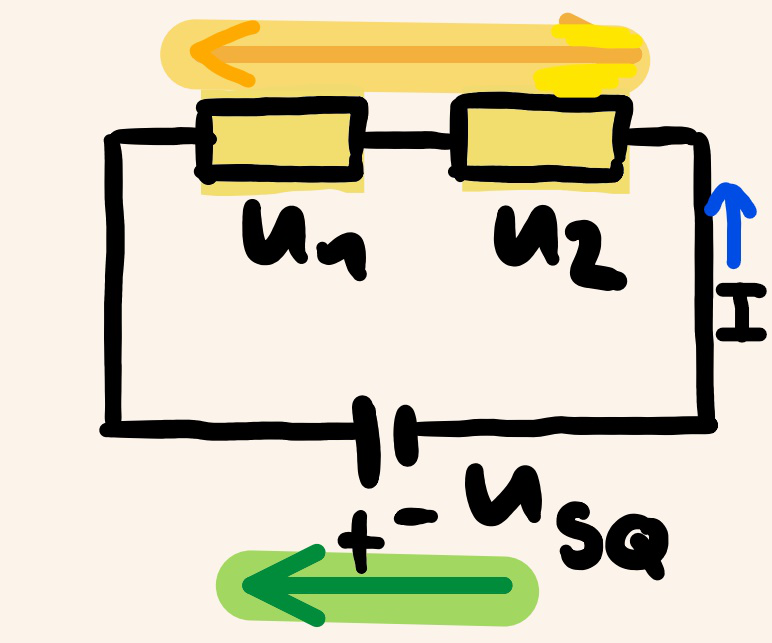
\includegraphics[width = 20mm]{src/images/maschenregel.png}
                \end{center}
            \end{footnotesize}
        \end{minipage}
        \begin{minipage}{0.5\linewidth}
            \begin{scriptsize}
                \begin{center}
                    \begin{align*}
                        \text{Widerstände:} \; &\sum\limits_{i} U_{i} = \sum\limits_k R_k I_k \\
                        \text{Kondensatoren:} \; &\sum\limits_{i} U_{i} = \sum\limits_k \frac{Q_k}{C_k} 
                    \end{align*}
                    $i =$ \# Spannungsquellen\\
                    $k =$ \# Spannungsabfälle
                \end{center}
                \vspace{1mm}
                \hfill \colorbox{YellowGreen}{$\sum U_\text{Quelle}$} $=$ \colorbox{Yellow}{$\sum U_\text{Abfälle}$} 
            \end{scriptsize}
        \end{minipage}
        \begin{scriptsize}
            (1) Zeichne \colorbox{YellowGreen}{$\vec{U}_{sq}$}an der Spannungsquelle ein (minus nach plus)
            \\(2) Wähle Stromrichtung \colorbox{Cyan}{$\vec{I}$} (gegen $U_{sq}$)
            \\(3) Trage \colorbox{Yellow}{$\vec{U}_R$} an Widerständen (ein gleich wie Stromrichtung)
        \end{scriptsize}
    \subsection{Schaltkreis}
    \vspace{-1mm}
    \begin{minipage}{0.49\linewidth}
        \begin{footnotesize}
            \begin{center}
                \vspace{2mm}
                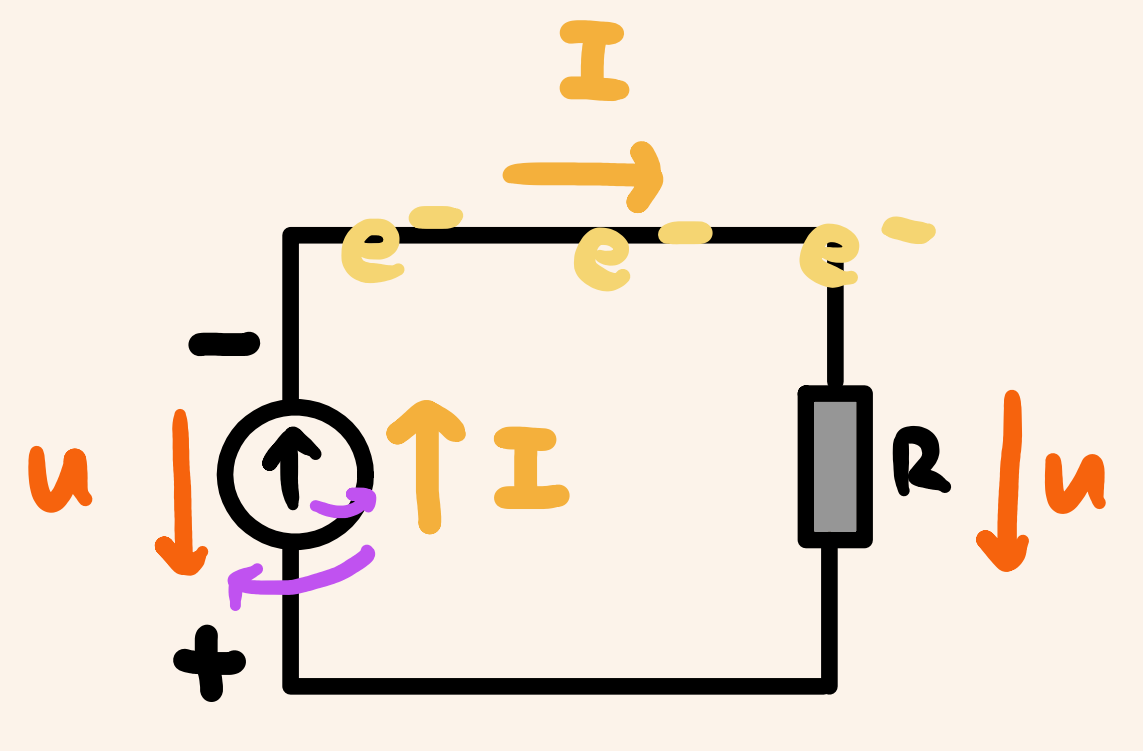
\includegraphics[width = 25mm]{src/images/schaltkreis.png}
            \end{center}
        \end{footnotesize}
    \end{minipage}
    \begin{minipage}{0.5\linewidth}
        \begin{scriptsize}
            \begin{center}
                \begin{align*}
                    \vec{I} = &\text{ Stromrichtung}
                    \\R = &\text{ Widerstand} 
                    \\\vec{U} = &\text{ Richtung des Spannungsabfall}
                    \\&\text{ Spannungsquelle: von mius nach plus}
                    \\&\text{ Widerstand: in Stromrichtung}
                \end{align*}
            \end{center}
        \end{scriptsize}
    \end{minipage}

    \subsubsection{Serieschaltung}
        \vspace{-1mm}
        \begin{minipage}{0.39\linewidth}
            \begin{footnotesize}
                \begin{center}
                    \vspace{2mm}
                    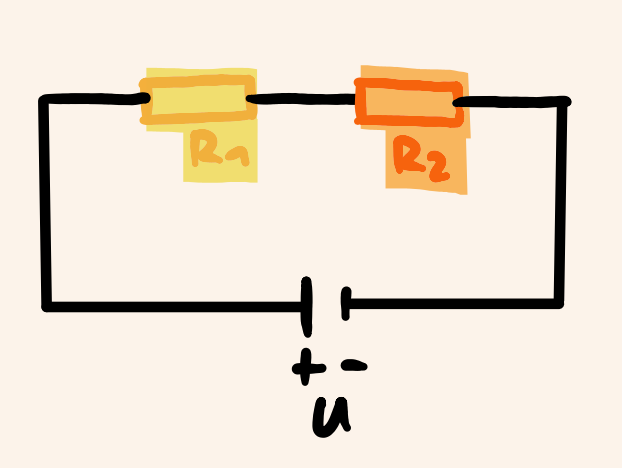
\includegraphics[width = 20mm]{src/images/serieschaltung.png}
                \end{center}
            \end{footnotesize}
        \end{minipage}
        \begin{minipage}{0.6\linewidth}
            \begin{scriptsize}
                \begin{center}
                    \begin{align*}
                        \text{Ladung:} \; Q_{\text{ges}} &= Q_i\\
                        \text{Stromstärke:} \; I_{\text{ges}} &= I_i\\
                        \text{Spannung:} \; U_{\text{ges}} &= \sum\limits_i U_i\\
                        \text{Widerstände:} \; R_{\text{res}} &= \sum\limits_i R_i\\
                        \text{Kondensatoren:} \; \frac{1}{C_{\text{res}}} &= \sum\limits_i \frac{1}{C_i}\\
                        \text{zwei Kondensatoren:} \; C_{res} &= \frac{C_1 \cdot C_2}{C_1 + C_2}
                    \end{align*}
                \end{center}
            \end{scriptsize}
        \end{minipage}
        \vspace{1mm}

    \subsubsection{Parallelschaltung}
        \vspace{-1mm}
        \begin{minipage}{0.39\linewidth}
            \begin{footnotesize}
                \begin{center}
                    \vspace{2mm}
                    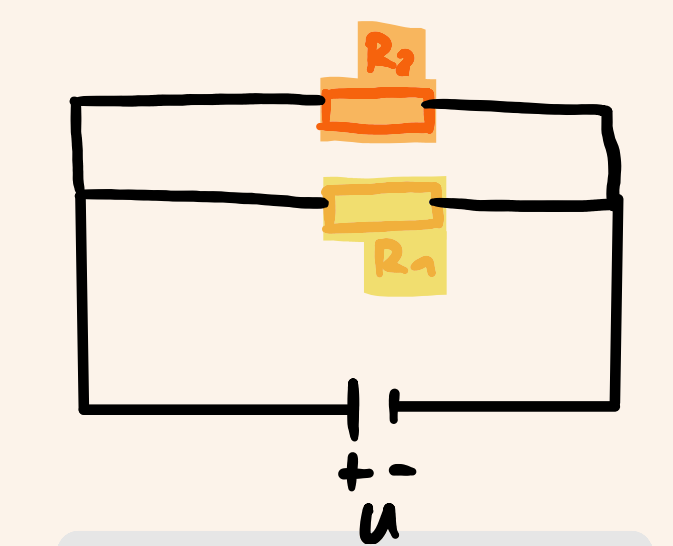
\includegraphics[width = 20mm]{src/images/parallelschaltung.png}
                \end{center}
            \end{footnotesize}
        \end{minipage}
        \begin{minipage}{0.6\linewidth}
            \begin{scriptsize}
                \begin{center}
                    \begin{align*}
                        \text{Ladung:} \; Q_{\text{ges}} &= \sum\limits_i Q_i\\
                        \text{Stromstärke:} \; I_{\text{ges}} &= \sum\limits_i I_i\\
                        \text{Spannung:} \; U_{\text{ges}} &= U_i\\
                        \text{Widerstände:} \; \frac{1}{R_{res}} &= \sum \frac{1}{R_i}\\
                        \text{zwei Widerstände:} \; R_{res} &= \frac{R_1 \cdot R_2}{R_1 + R_2}\\
                        \text{Kondensatoren:} \; C_{res} &= \sum\limits_i C_i
                    \end{align*}
                \end{center}
            \end{scriptsize}
        \end{minipage}
    \subsection{Strom/Spannnungsteiler}
    Spannungsteiler (Kondensator/Widerstand):\\
    \begin{minipage}{0.49\linewidth}
        \begin{center}
            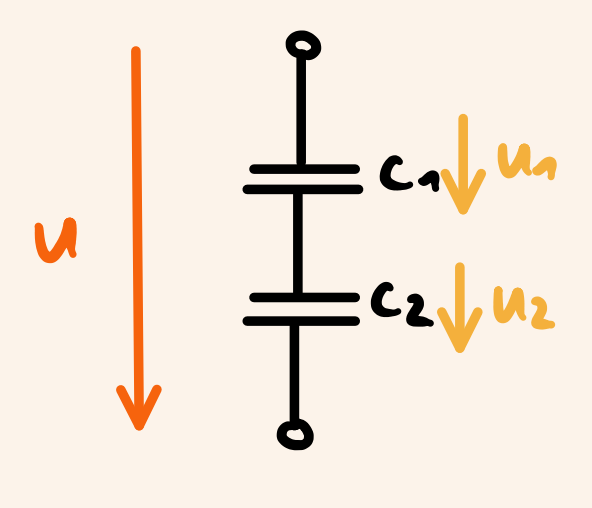
\includegraphics[width = 0.49\linewidth]{src/images/Spannungsteiler_1.png}
        \end{center}
    \end{minipage}
    \begin{minipage}{0.49\linewidth}
        \begin{center}
            \begin{empheq}[box=\fbox]{align*}
                U^C_1 = U \cdot \frac{C_2}{C_1 + C_2}\\
                U^C_2 = U \cdot \frac{C_1}{C_1 + C_2}\\
                U^R_1 = U \cdot \frac{R_1}{R_1 + R_2}\\
                U^R_2 = U \cdot \frac{R_2}{R_1 + R_2}
            \end{empheq}
        \end{center}
    \end{minipage}

    Stromteiler:\\
    \begin{minipage}{0.49\linewidth}
        \begin{center}
            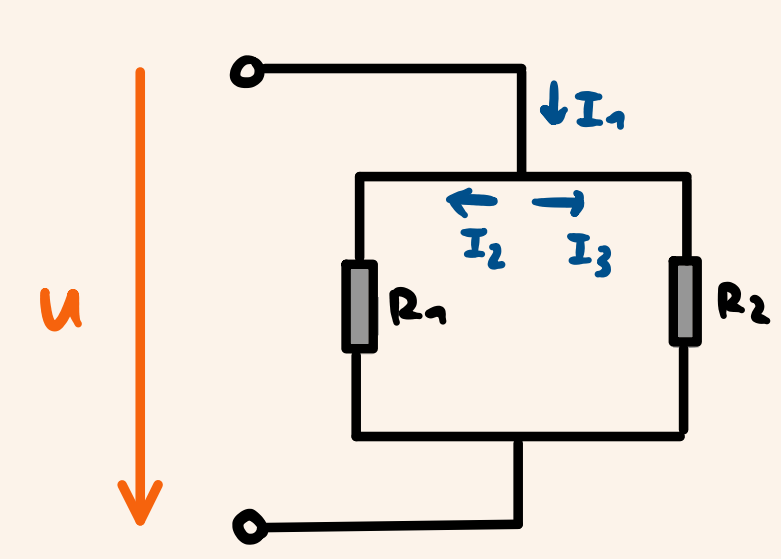
\includegraphics[width = 0.49\linewidth]{src/images/Stromteiler.png}
        \end{center}
    \end{minipage}
    \begin{minipage}{0.49\linewidth}
        \begin{center}
            \begin{empheq}[box=\fbox]{align*}
                I_1 = I \cdot \frac{R_1}{R_1 + R_2}\\
                I_2 = I \cdot \frac{R_2}{R_1 + R_2}
            \end{empheq}
        \end{center}
    \end{minipage}
    \vfill \null \columnbreak

\section{Elektrostatik}
    \subsection{Elektrisches Feld}
    \begin{tabular}{l|l l}
        Homogenes Feld & Inhomogenes Feld & 
        \\(Plattenkondensator) & (Punktladung) & 
        \\
        \\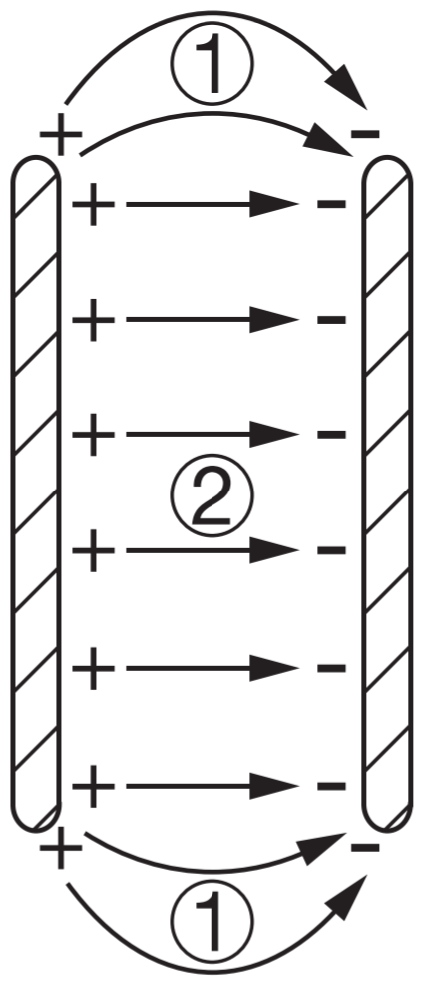
\includegraphics[width = 10mm]{src/images/kondensator.png} & 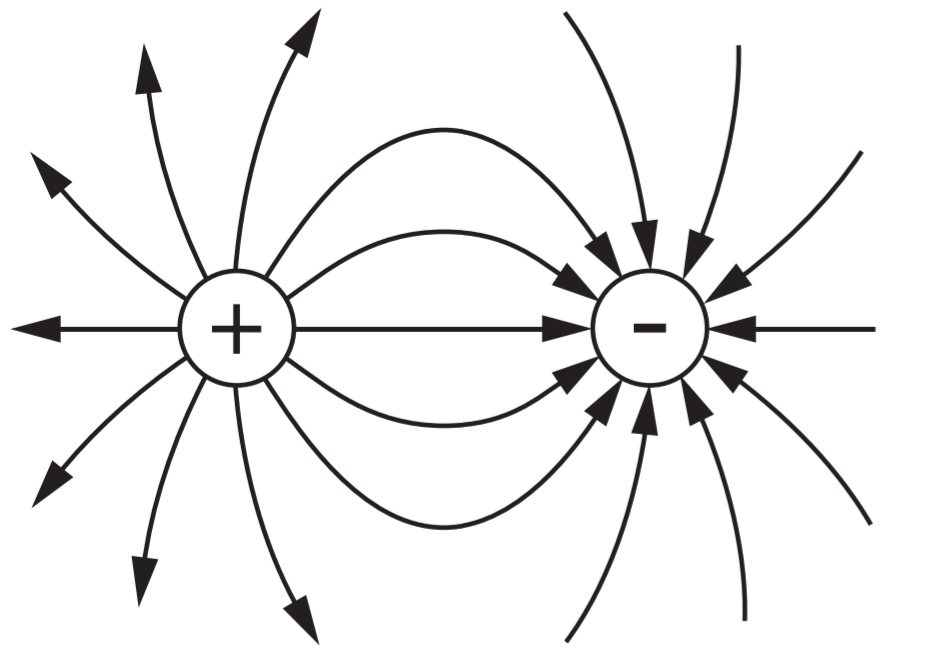
\includegraphics[width = 21mm]{src/images/zwei_punktladung.png} & 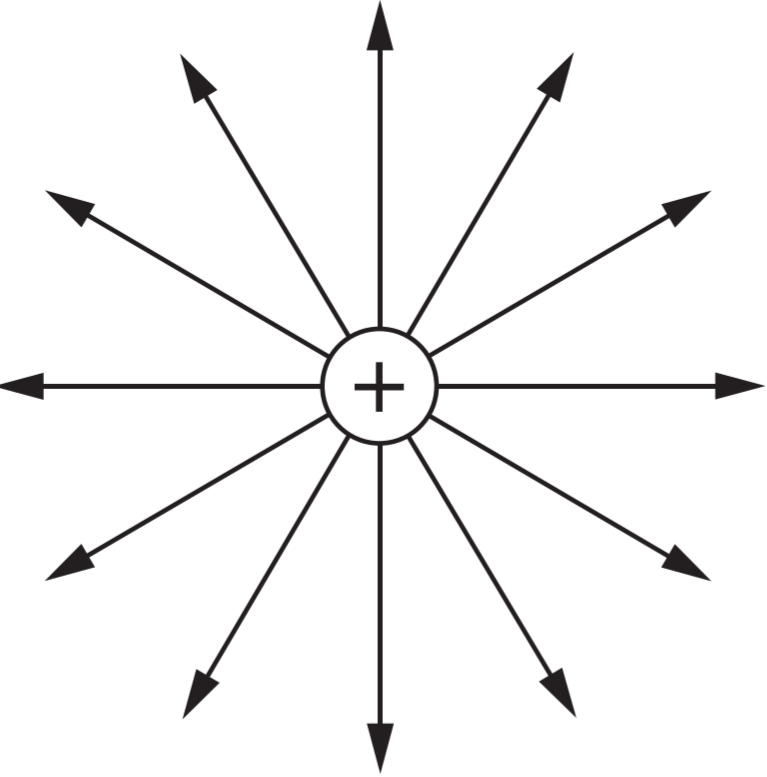
\includegraphics[width = 15mm]{src/images/punktladung.png}
    \end{tabular}
    \vspace{2mm}

    Quick facts:
    \begin{itemize}
        \item Jede Ladung erzeugt ein $E$ - Feld \vspace{-1mm}
        \item Feldlinien von + nach - \vspace{-1mm}
        \item Feldlinien immer $\bot$ auf leitfähigen Körpern \vspace{-1mm}
        \item Feldlinien schneiden sich nie \vspace{-1mm}
        \item Innerhalb von Leitern gibt es kein Feld
    \end{itemize}


    \input{src/2_elektrostatik/2_elektrische_feldstärke.tex}
    \subsubsection{Elektrische Flussdichte/Verschiebungsdichte D}
    \begin{minipage}{0.49\linewidth}
        \begin{center}
            Dichte der Ladung:\\
            \mathbox{\vec{D} = \frac{Q}{A} \vec{e}}
        \end{center}
    \end{minipage}
    \begin{minipage}{0.49\linewidth}
        \begin{center}
                \mathbox{\vec{D} = \varepsilon \cdot \vec{E}}
                $\varepsilon = \varepsilon_0 \cdot \varepsilon_r$
        \end{center}
    \end{minipage}
    \vspace{0em}
    \subsubsection{Elektrisches Potential $\Phi$}
    \begin{center}
        \begin{tabular}{c c}
            Allgemein: & Punktladung:\\
            $\Phi(P) = -\int \vec{E} \vec{ds}$ & $\Phi(r) = \frac{1}{4 \pi \varepsilon_0} \frac{q_1}{r}$
        \end{tabular}
    \end{center}
    \subsubsection{Elektrische Spannung U \hfill $[V]$}
        Inhomogen:
        \mathbox{U = \Phi(P) - \Phi(P_0) = -\int\limits_{P_0}^{P} \vec{E}\vec{ds}}
            
        Homogen:

        \vspace{-1mm}
            \begin{minipage}{0.41\linewidth}
                \begin{footnotesize}
                    \begin{center}
                        \vspace{2mm}
                        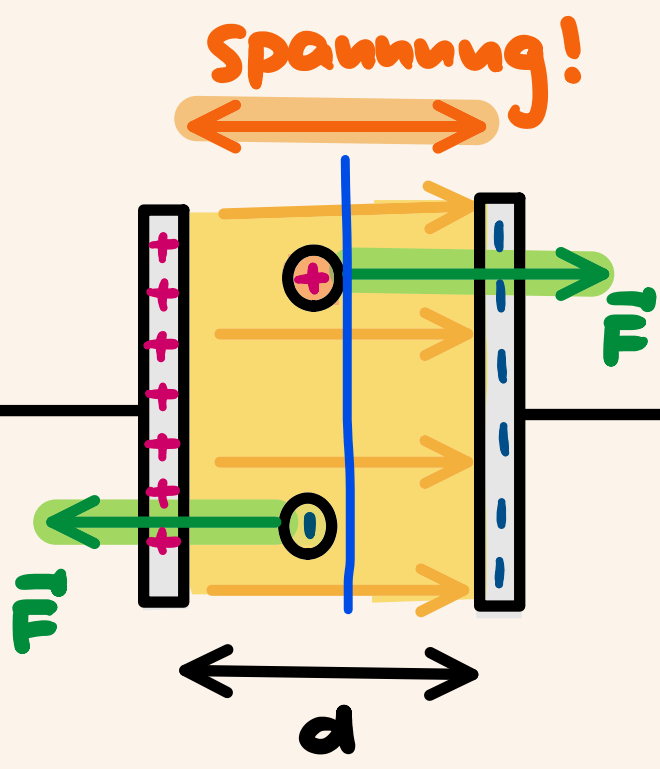
\includegraphics[width = 15 mm]{src/images/hom_potentialfeld.png}
                    \end{center}
                \end{footnotesize}
            \end{minipage}
            \begin{minipage}{0.58\linewidth}
                \begin{scriptsize}
                    \begin{center}
                        \mathbox{
                            U = E\cdot d
                        }
                        Auf \colorbox{Cyan}{Linie} stets selbes Potential/Spannung
                    \end{center}
                \end{scriptsize}
            \end{minipage}
            \vspace{1mm}
    \subsubsection{Elektrisches Dipolmoment}
    Für zwei gleich stark, mit unterschiedlichem Vorzeichen geladene Ladungen:\\
    \begin{minipage}{0.59\linewidth}
        \begin{empheq}[box = \fbox]{align*}
            \vec{p} &= Q \vec{l}\\
            \vec{E_{dip}} &= \frac{1}{4 \pi \varepsilon_0} \frac{3 (\vec{p} \hat{r}) \hat{r} - \vec{p}}{r^3}
        \end{empheq}
    \end{minipage}
    \begin{minipage}{0.39\linewidth}
        \begin{scriptsize}
            Variablen erklären
        \end{scriptsize}
    \end{minipage}

    \subsection{Elektrischer Fluss $\Psi$} \label{Gauss'sches Gesetz E}
    \begin{minipage}{0.49\linewidth}
        \mathbox{
            \Psi = \int \vec{E} d \vec{A}
        }
    \end{minipage}
    \begin{minipage}{0.49\linewidth}
        \begin{scriptsize}
            $E$ = Elektrisches Feld\\
            $A$ = Fläche, durch die das Feld hindurchfliesst
        \end{scriptsize}
    \end{minipage}

    \begin{minipage}{0.54\linewidth}
        \begin{empheq}[box = \fbox]{align*}
            \oint \vec{E} \vec{dA} = \frac{1}{\varepsilon_0} \int \rho dV = \frac{Q}{\varepsilon_0}\\
            div(\vec{E}) = \frac{1}{\varepsilon_0} \rho
        \end{empheq}
    \end{minipage}
    \begin{minipage}{0.44\linewidth}
        \begin{scriptsize}
            Mittels dem Satz von Gauss erhält man die erste Maxwell Gleichung\\
            $\rho$ = Ladungsdichte\\
            $Q$ = Gesamtladung innerhalb der Fläche
        \end{scriptsize}
    \end{minipage}

    
    \subsection{Kraft, Arbeit, Leistung}
    \subsubsection{Kraft im $\vec{E}$ Feld \hfill $[N]$}
        \mathbox{\vec{F_E} = Q \vec{E_0}}
    
    \subsubsection{pot. Energie von Ladungen \hfill $[J]$}
        \begin{minipage}{0.49\linewidth}
            \begin{empheq}[box = \fbox]{align*}
                E_{pot} &= Q \Phi\\
                &= Q \int \vec{E} d \vec{s}
            \end{empheq}
            Im Plattenkondensator:
            \begin{empheq}[box = \fbox]{align*}
                E_{pot} &= Q \cdot E \cdot l\\
                &= Q \cdot U
            \end{empheq}
        \end{minipage}
        \begin{minipage}{0.49\linewidth}
            \begin{scriptsize}
                \begin{empheq}{align*}
                    Q = &\text{Ladung}\\
                    U = &\text{Spannung}\\
                    \Phi = &\text{el. Potential}\\
                    E = &\text{el. Feldstärke}\\
                    l = &\text{Entfernung zwischen}\\
                    &\text{Kondensatorflächen}\\
                \end{empheq}
            \end{scriptsize}
        \end{minipage}    
    
    %\vfill \null \columnbreak

    \subsubsection{Arbeit im $\vec{E}$ Feld \hfill $[J]$}
        Die gespeicherte Energie ist jeweils die verrichtete Arbeit: $\Delta E = W$
        Arbeit $=$ Kraft $\cdot$ Weg
        \begin{empheq}[box = \fbox]{align*}
            W &= \int \vec{F}d\vec{s} = \int \vec{E} \cdot Q d\vec{s} = Q \Delta \Phi\\
            &= Q U = C U^2 = U \cdot I \cdot t\\
            dW &= UI dt
        \end{empheq}
        \begin{center} \underline{\textbf{Gespeicherte Energie im Kondensator:}} \end{center}
        \begin{minipage}{0.49\linewidth}
            \begin{itemize}
                \item Energie entspricht Fläche unter Q-U-Diagramm.
                \item Ladevorgang eines Kondensators verläuft linear.
                \item Somit: Energie entspricht Dreiecksfläche mit Seitenlänge Ladung und Spannung nach Ladevorgang.
            \end{itemize}
        \end{minipage}
        \begin{minipage}{0.49\linewidth}
            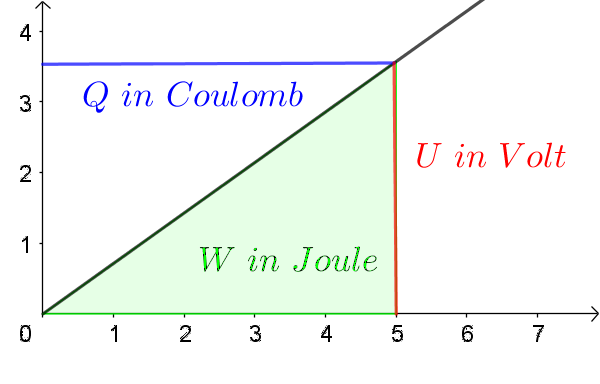
\includegraphics[width = 1\linewidth]{src/images/ladevorgang_kondensator.png}
        \end{minipage}

        \begin{minipage}{0.69\linewidth}
            \begin{empheq}[box = \fbox]{align*}
                W &= \int U dq = \frac{Q U}{2} =  \frac{Q^2}{2C} = \frac{CU^2}{2}\\
                &= \frac{1}{2} \varepsilon_0 E_0^2 V\\
                \rho_{el} &= \frac{W}{V} = \frac{1}{2} \varepsilon_0 E_0^2
            \end{empheq}
        \end{minipage}
        \begin{minipage}{0.29\linewidth}
            \begin{scriptsize}
                \begin{empheq}{align*}
                    Q = &\text{Ladung}\\
                    U = &\text{Spannung}\\
                    C = &\text{Kapazität}\\
                    E_0 = &\text{Elektrische Feldstärke}\\
                    V = &\text{Volumen zwischen}\\
                    &\text{Kondensatorflächen}\\
                    \rho_{el} = &\text{Energiedichte}
                \end{empheq}
            \end{scriptsize}
        \end{minipage}
    \vfill \null \columnbreak

    \subsubsection{Leistung im $\vec{E}$ Feld \hfill $\left[\frac{J}{s}\right]$}
        \mathbox{P = \frac{W}{t} = F \cdot v = U \cdot I}
    

\section{Magnetisches Feld}
    \input{src/3_magnetisches_feld/1_feldstärke.tex}
    \subsection{Magnetische Flussdichte B \hfill $[T]$}
    \begin{minipage}{0.49\linewidth}
        \begin{empheq}[box = \fbox]{align*}
            B = \frac{\Phi}{A} = \mu H
        \end{empheq}  
    \end{minipage}
    \begin{minipage}{0.49\linewidth}
        \begin{scriptsize}
            \begin{empheq}{align*}
                \mu &= \mu_0 \cdot \mu_r = \text{Mag. Permeabilität}\\
                A &= \text{Durchflossene Fläche}\\
                H &= \text{Mag. Feldstärke}\\
                \Phi &= \text{Mag. Fluss}
            \end{empheq}
        \end{scriptsize}
    \end{minipage}
    \vspace{2mm}

    \begin{minipage}{0.49\linewidth}
        \centering \underline{\textbf{Langer Leiter}}\\
        \begin{empheq}[box = \fbox]{align*}
            B = \frac{\mu\mu_0 I}{2 \pi r}
        \end{empheq}  
    \end{minipage}
    \begin{minipage}{0.49\linewidth}
        \centering \underline{\textbf{Spule}}\\
        \begin{empheq}[box = \fbox]{align*}
            B = \mu\mu_0  I \frac{n}{l}
        \end{empheq}  
    \end{minipage}
    \subsection{Magnetischer Fluss $\Phi$ \hfill $[T m^2]$}
    \begin{minipage}{0.49\linewidth}
        \begin{empheq}[box = \fbox]{align*}
            \Phi &= \mu A H\\
            &=\int \vec{B} \vec{dA}
        \end{empheq}  
    \end{minipage}
    \begin{minipage}{0.49\linewidth}
        \begin{scriptsize}
            \begin{empheq}{align*}
                \mu &= \mu_0 \cdot \mu_r = \text{Mag. Permeabilität}\\
                A &= \text{Durchflossene Fläche}\\
                H &= \text{Mag. Feldstärke}\\
                B &= \text{Mag. Flussdichte}
            \end{empheq}
        \end{scriptsize}
    \end{minipage}
    

    \subsection{Magnetisches Dipolmoment}
    \begin{minipage}{0.49\linewidth}
        \begin{empheq}[box = \fbox]{align*}
            \vec{m} = I \vec{A}
        \end{empheq}  
    \end{minipage}
    \begin{minipage}{0.49\linewidth}
        \begin{scriptsize}
            \begin{empheq}{align*}
                I &= \text{el. Strom}\\
                \vec{A} &= \text{Vektor normal zu durchflossener Fläche}\\
            \end{empheq}
        \end{scriptsize}
    \end{minipage}
    \input{src/3_magnetisches_feld/5_induktivität.tex}
    \subsection{elektromagnetische Induktion}
    \centering \underline{\textbf{Spannungsstoss $S_U$}}\\
    Änderung des magnetischen Feldes erzeugt Strom in Spule
    \begin{minipage}{0.44\linewidth}
        \begin{empheq}[box = \fbox]{align*}
            S_U &= \int U_i dt\\
            &= \mu n_i \Delta H A_i
        \end{empheq}  
    \end{minipage}
    \begin{minipage}{0.54\linewidth}
        \begin{scriptsize}
            \begin{empheq}{align*}
                \mu &= \mu_0 \cdot \mu_r = \text{Mag. Permeabilität}\\
                U_i &= \text{Spannung in der Spule i}\\
                n_i &= \text{Windungen der Spule i}\\
                H &= \text{Mag. Feldstärke}\\
                A_i &= \text{Querschnittsfläche der Spule i}\\
            \end{empheq}
        \end{scriptsize}
    \end{minipage}
    
    \centering \underline{\textbf{Induktionsgesetz}}\\ \label{Induktionsgesetz}
    \begin{minipage}{0.58\linewidth}
        \begin{empheq}[box = \fbox]{align*}
            U_i &= -n_i \frac{d\Phi}{dt}\\
            &= \underbrace{-n_i \frac{d}{dt} \iint \vec{B}\vec{dA}}_{\text{$\vec{B}$ hom. auf $A$ und $\vec{B} \| \vec{dA}$,}}\\
            &= -n_i B A
        \end{empheq}
    \end{minipage}
    \begin{minipage}{0.40\linewidth}
        \begin{scriptsize}
            Minus wegen Lenzscher Regel
            \begin{empheq}{align*}
                U_i &= \text{Induzierte Spannung in Spule}\\
                n_i &= \text{Windungen der Spule i}\\
                \Phi &= \text{Mag. Fluss}\\
                B &= \text{mag. Flussdichte}\\
                A &= \text{Querschnittsfläche Spule,}\\ 
                &\text{normal zu Fläche}
            \end{empheq}
        \end{scriptsize}
    \end{minipage}

    \centering \underline{\textbf{Induktionsspule}}\\
    \begin{minipage}{0.44\linewidth}
        \begin{empheq}[box = \fbox]{align*}
            \int U_i dt &= \alpha \int \vec{H} \cdot \vec{ds}\\
            \alpha &= \mu \frac{n_i}{l} A_i\\
            B &= \frac{L I}{n A}
        \end{empheq}
    \end{minipage}
    \begin{minipage}{0.54\linewidth}
        \begin{scriptsize}
            \begin{empheq}{align*}
                U_i &= \text{Spannung in der Spule i}\\
                \vec{H} &= \text{magnetische Feldstärke}\\
                \mu &= \mu_0 \cdot \mu_r = \text{Mag. Permeabilität}\\
                n_i &= \text{Windungen der Spule i}\\
                l &= \text{Länge der Spule}\\
                B &= \text{mag. Flussdichte}\\
                L &= \text{Induktivität}\\
                A &= \text{Querschnittsfläche Spule, normal zu Fläche}
            \end{empheq}
        \end{scriptsize}
    \end{minipage}

    \subsubsection{Selbstinduktion}
    \begin{minipage}{0.49\linewidth}
        \mathbox{U_i = -L \frac{dI}{dt}}
        \begin{scriptsize}
            \begin{empheq}{align*}
                U_i &= \text{induzierte Spannung}\\
                L &= \text{Induktivität}\\
                I &= \text{el. Strom}
            \end{empheq}
        \end{scriptsize}
    \end{minipage}
    \begin{minipage}{0.49\linewidth}
        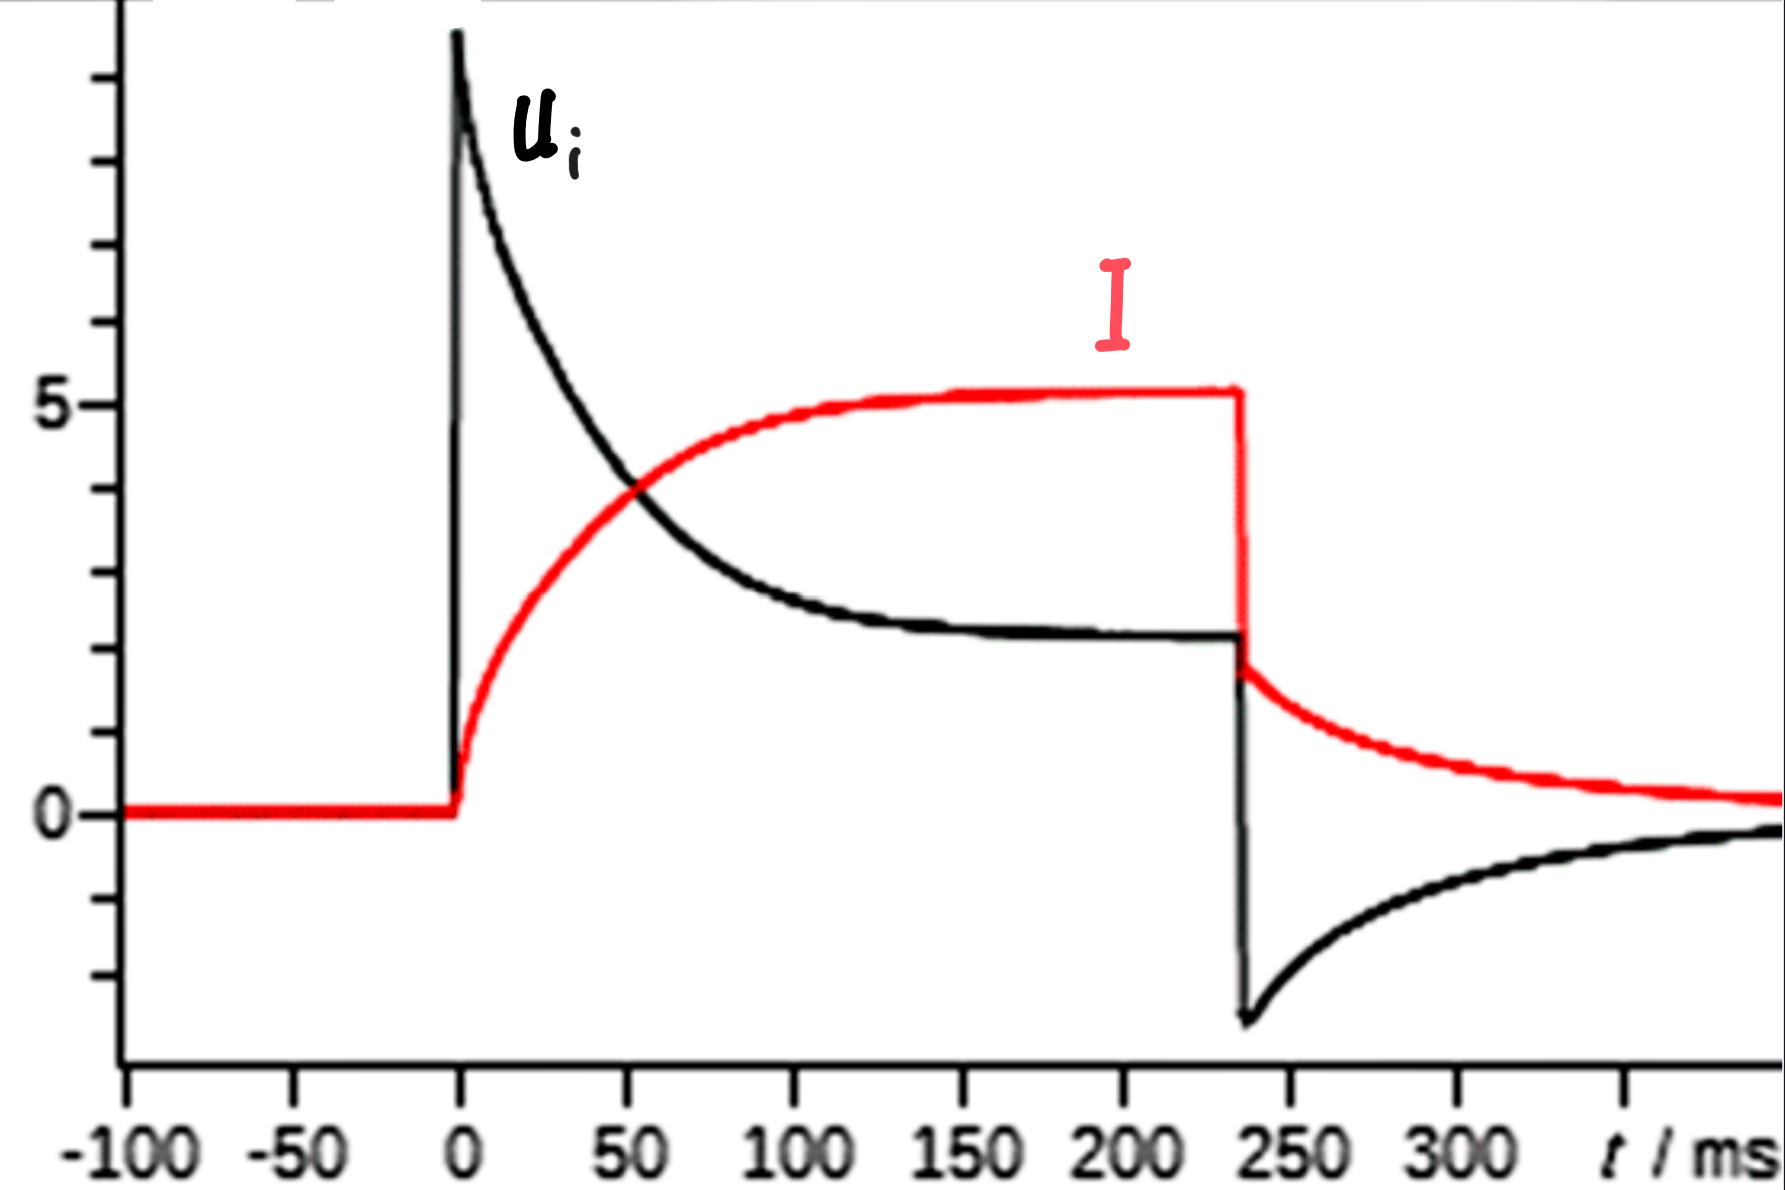
\includegraphics[width = \linewidth]{src/images/selbstinduktion.png}
    \end{minipage}
    
    \subsubsection{Gegeninduktion}
    \begin{minipage}{0.54\linewidth}
        \begin{empheq}[box = \fbox]{align*}
            U_{i2} &= L_{12} \frac{dI_1}{dt}\\
            L_{12} &= L_{21}
        \end{empheq}
        Übereinanderliegende Spulen gleicher Länge bzw. Fläche:\\
        \begin{empheq}[box = \fbox]{align*}
            L_{12} &= n_2 \frac{\Phi_1}{I_1} = \mu_0 n_1 n_2 \frac{A_1}{l_1}
        \end{empheq}
    \end{minipage}
    \begin{minipage}{0.44\linewidth}
        \begin{itemize}
            \item Feldspule$_1$: Spannung per Batterie
            \item Induktionsspule$_2$: Induzierte Spannung
        \end{itemize}
        \begin{scriptsize}
            \begin{empheq}{align*}
                U &= \text{el. Spannung}\\
                L &= \text{Induktivität}\\
                n &= \text{Windungen der Spule}\\
                \Phi &= \text{mag. Fluss durch Spule}\\
                A &= \text{Querschnittsfläche Spule}\\
                l &= \text{Länge Spule}\\
            \end{empheq}
        \end{scriptsize}
    \end{minipage}

    
    \subsection{Lenzsche Regel}
    \begin{itemize}
        \item System reagiert der zeitlichen Änderung des magnetischen Feldes entgegen / wehrt sich gegen Änderung des magnetischen Feldes
        \item Bedingung: Strom muss in System fliessen können (Bsp metallischer Ring ohne Lücken)
        \item Richtung des induzierten Feldes entgegengesetzt der Richtung der Änderung des äusseren Feldes.
    \end{itemize}
%
    \centering Aus Induktionsgesetz folgt:\\
    \begin{minipage}{0.49\linewidth}
        \begin{empheq}[box = \fbox]{align*}
            \oint \vec{E} \vec{ds} &= -\frac{d}{dt} \int \vec{B} \vec{dA}\\
            rot(\vec{E}) &= -\dot{\vec{B}}
        \end{empheq}
    \end{minipage}
    \begin{minipage}{0.49\linewidth}
        \begin{scriptsize}
            \begin{empheq}{align*}
                \vec{E} &= \text{Elektrische Feldstärke}\\
                \vec{B} &= \text{Magnetische Flussdichte}\\
            \end{empheq}
        \end{scriptsize}
    \end{minipage}
    \subsection{Durchflutungsgesetz} \label{Durchflutungsgesetz}
    \begin{minipage}{0.64\linewidth}
        \begin{empheq}[box = \fbox]{align*}
            \begin{array}{r@{\ }l} %{r@{\ }c@{\ }l}
                \oint\limits \vec{H} ds &= n \cdot I_{tot}\\
                &= \int \vec{j} + \frac{\vec{dD}}{dt} \vec{dA}\\
                rot(\vec{H}) &= \vec{j} + \dot{\vec{D}}
            \end{array}
        \end{empheq}  
    \end{minipage}
    \begin{minipage}{0.34\linewidth}
        \begin{scriptsize}
            \begin{empheq}{align*}
                \vec{H} &= \text{mag. Feldstärke}\\
                I &= j \cdot A = \text{el. Strom}\\
                j &= \text{Stromflächendichte}\\
                D &= \text{el. Flussdichte}
            \end{empheq}
        \end{scriptsize}
    \end{minipage}
    \subsection{Lorenzkraft $\vec{F_L}$}
    \begin{minipage}{0.49\linewidth}
        \begin{empheq}[box = \fbox]{align*}
            \vec{F_L} &= \underbrace{I (\vec{l} \times \vec{B})}_{\text{falls $\vec{I}, \vec{l} $und$ \vec{B}\bot $ }}\\
            &= I \cdot l \cdot B \\
            \vec{F_L} &= \int \vec{j} \times \vec{B} dV\\
            &= \int \rho (\vec{v} \times \vec{B}) dV\\
            &= q (\vec{v} \times \vec{B})
        \end{empheq}
        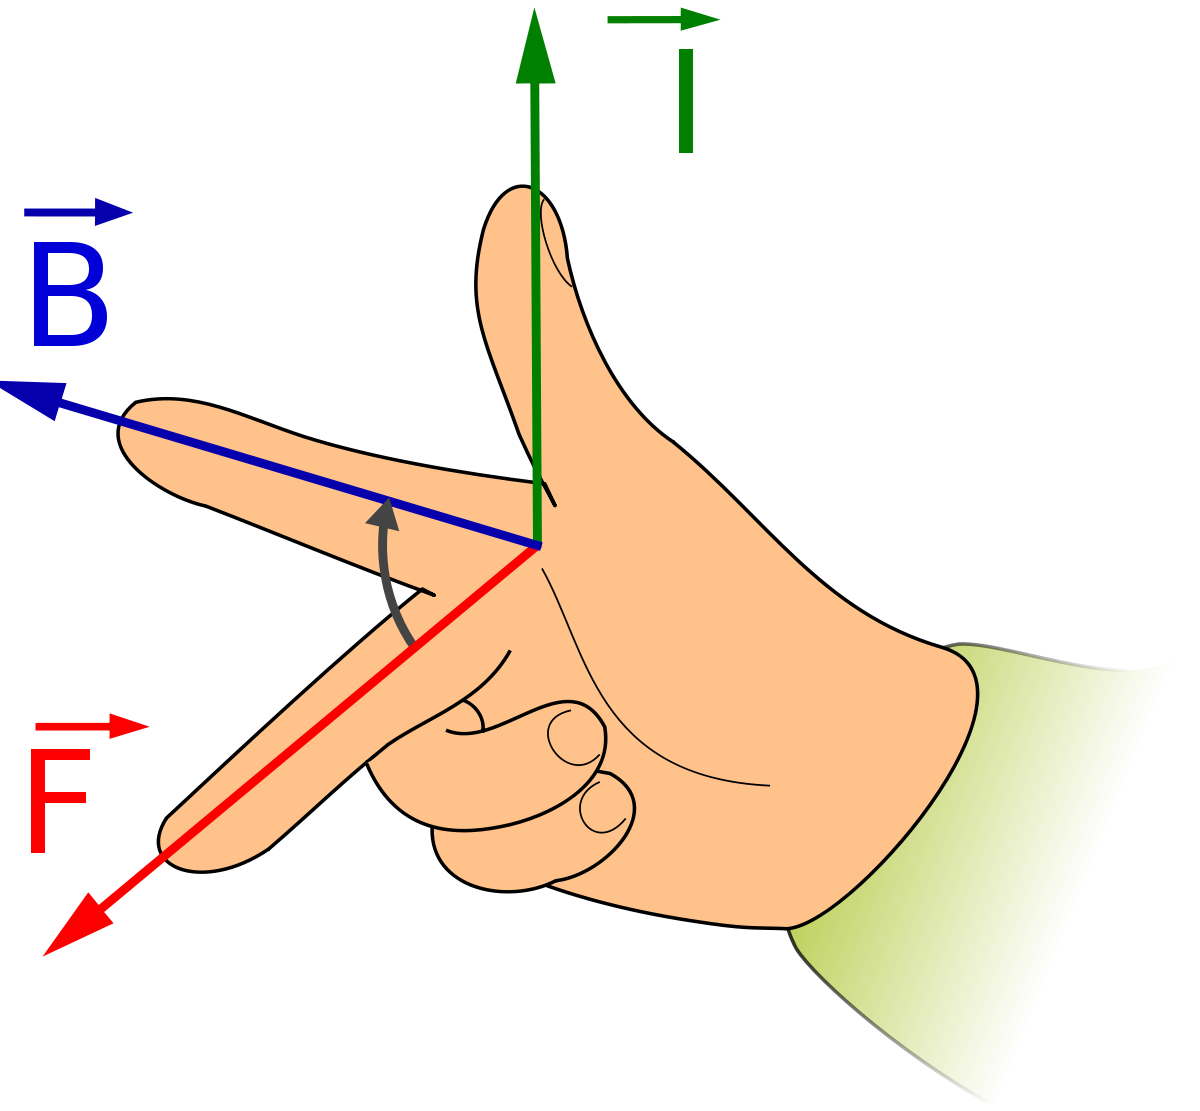
\includegraphics[width = \linewidth]{src/images/rechte_hand_lorenz.png}
    \end{minipage}
    \begin{minipage}{0.49\linewidth}
        \begin{scriptsize}
            \begin{empheq}{align*}
                l = &\text{Länge stromdurchflossener}\\
                &\text{Leiter in Magnetfeld}\\
                A = &\text{Querschnittsfläche Leiter}\\
                V = &A \cdot l = \text{Volumen Leiter}\\
                j = &\frac{I}{A} = \text{Flächenstromdichte}\\
                \rho = &\text{Volumenladungsdichte}\\
                \vec{B} = &\text{Magnetfeld}\\
                I = &\rho A v = \text{el. Strom}\\
                v = &\text{Geschwindigkeit der Ladungen}\\
                q = &\text{Ladung !Vorzeichen!}
            \end{empheq}
            \linebreak
            ACHTUNG: Richtung Bild = Richtung technischer Strom! Elektronenfluss in entgegengesetzte Richtung zu Fluss des technischen Stroms
        \end{scriptsize}
    \end{minipage}
    \subsection{Biot-Savart Gesetz} \label{sec_biot_savart}
    Magnetische Wirkung eines Abschnittes eines elektrischen Leiters $\vec{dl}$ auf einen Punkt im Abstand $\left|\vec{r}\right|$   
    \mathbox{\vec{B} = \frac{\mu_0}{4 \pi} \int \frac{I \vec{dl} \times \hat{r}}{r^2}}

    \subsection{Energie im magnetischen Feld}
    \begin{minipage}{0.49\linewidth}
        \begin{empheq}[box = \fbox]{align*}
            E_p &= \int_0^{\infty} -U_i I dt\\
            %&= \int_0^{\infty} L \frac{dI}{dt} I dt\\
            &= \frac{1}{2} L I_0^2\\
            %&= \frac{1}{2} \mu_0 n^2 \frac{A}{l} I_0^2\\
            &= \frac{1}{2} \mu_0 V H^2\\
            \rho_m &= \frac{W}{V} = \frac{\vec{B} \vec{H}}{2}
        \end{empheq}
    \end{minipage}
    \begin{minipage}{0.49\linewidth}
        \begin{scriptsize}
            \begin{empheq}{align*}
                P &= U \cdot I = \frac{W}{t} = -P_i = -U_i \cdot I\\
                U &= \text{el. Spannung}\\
                I &= \text{el. Strom}\\
                P &= \text{Leistung}\\
                L &= \text{Induktivität Spule}\\
                V &= \text{Eingeschlossenes Volumen der Spule}\\
                H &= \text{mag. Feldstärke}\\
                B &= \text{mag. Flussdichte}\\
                \rho_m &= \text{Volumenenergiedichte}\\
            \end{empheq}
        \end{scriptsize}
    \end{minipage}
    \subsection{Maxwell Gleichungen}
    \begin{align*}
        \parbox{3.5cm}{\textbf{Gauss'sches Gesetz $\vec{E}$} \ref{Gauss'sches Gesetz E}}\\
        \vec{\nabla}\vec{E}(\vec{r}) &= \frac{\rho{\vec{r}}}{\varepsilon_0}\\
        \int_{\partial V} \vec{E}(\vec{r}) d \vec{A} &= \frac{1}{\varepsilon_0} \int_V \rho(\vec{r}) dV
        \\[0.5em]
        \parbox{3.5cm}{\textbf{Gauss'sches Gesetz $\vec{B}$}}\\
        \vec{\nabla}\vec{B}(\vec{r}) &= 0\\
        \oint_{\partial V} \vec{B}(\vec{r}) d \vec{A} &= 0
        \\[0.5em]
        \parbox{3.5cm}{\textbf{Induktionsgesetz} \ref{Induktionsgesetz}}\\
        \vec{\nabla} \times \vec{E}(\vec{r},t) &= - \frac{\partial \vec{B}(\vec{r},t)}{\partial t}\\
        U_\text{ind} = \oint_L \vec{E}_\text{ind}(\vec{r}) d \vec{L} &= - \frac{d}{dt} \int_A \vec{B}(\vec{r}) d \vec{A}
        \\[0.5em]
        \parbox{3.5cm}{\textbf{Durchflutungsgesetz} \ref{Durchflutungsgesetz}}\\
        \vec{\nabla} \times \vec{B}(\vec{r}) &= \mu_0 \vec{j}(\vec{r}) + \mu_0 \varepsilon_0 \frac{\partial \vec{E}(\vec{r})}{\partial t}\\
        \oint_L \vec{B}(\vec{r}) d \vec{L} &= \mu_0 \int_A \vec{j}(\vec{r}) d \vec{A}
    \end{align*}
    \vfill \null \columnbreak
    \subsection{Magnetismus der Materie}
    Magnetische Suszeptibilität:
    \mathbox{X = \mu - 1}

    Magnetisierung:
    \mathbox{\vec{M} = X \vec{H}}
    \begin{itemize}
        \item paramagnetische Materialien: $X > 0$, Magnetisierung in gleiche Richtung wie Feld. 
        \item diamagnetische Materialien: $X < 0$, Magnetisierung in entgegengesetzte Richtung wie Feld.
    \end{itemize}

    Elektronen bewegen sich auf einer Kreisbahn im Atom -> magnetisches Moment entsteht. Bei angelegtem magnetischem Feld werden die magnetischen Momente aller Atome parallel ausgerichtet
    \textbf{Schema mit magnetischem Moment einfügen}

    Hysterese: Wenn nach der Magnetisierung eines ferromagnetischen Materials das magnetische Feld wieder ausgeschalten wird, setzt ein "Memory-Effekt ein.
    Eine verbleibende magnetische Wirkung im Material bezeichnet man als \textbf{Remanenz}.
    Das Feld, welches benötigt wird, um die Remanenz auszulöschen, bezeichnet man als \textbf{Hoerzitivkraft}
    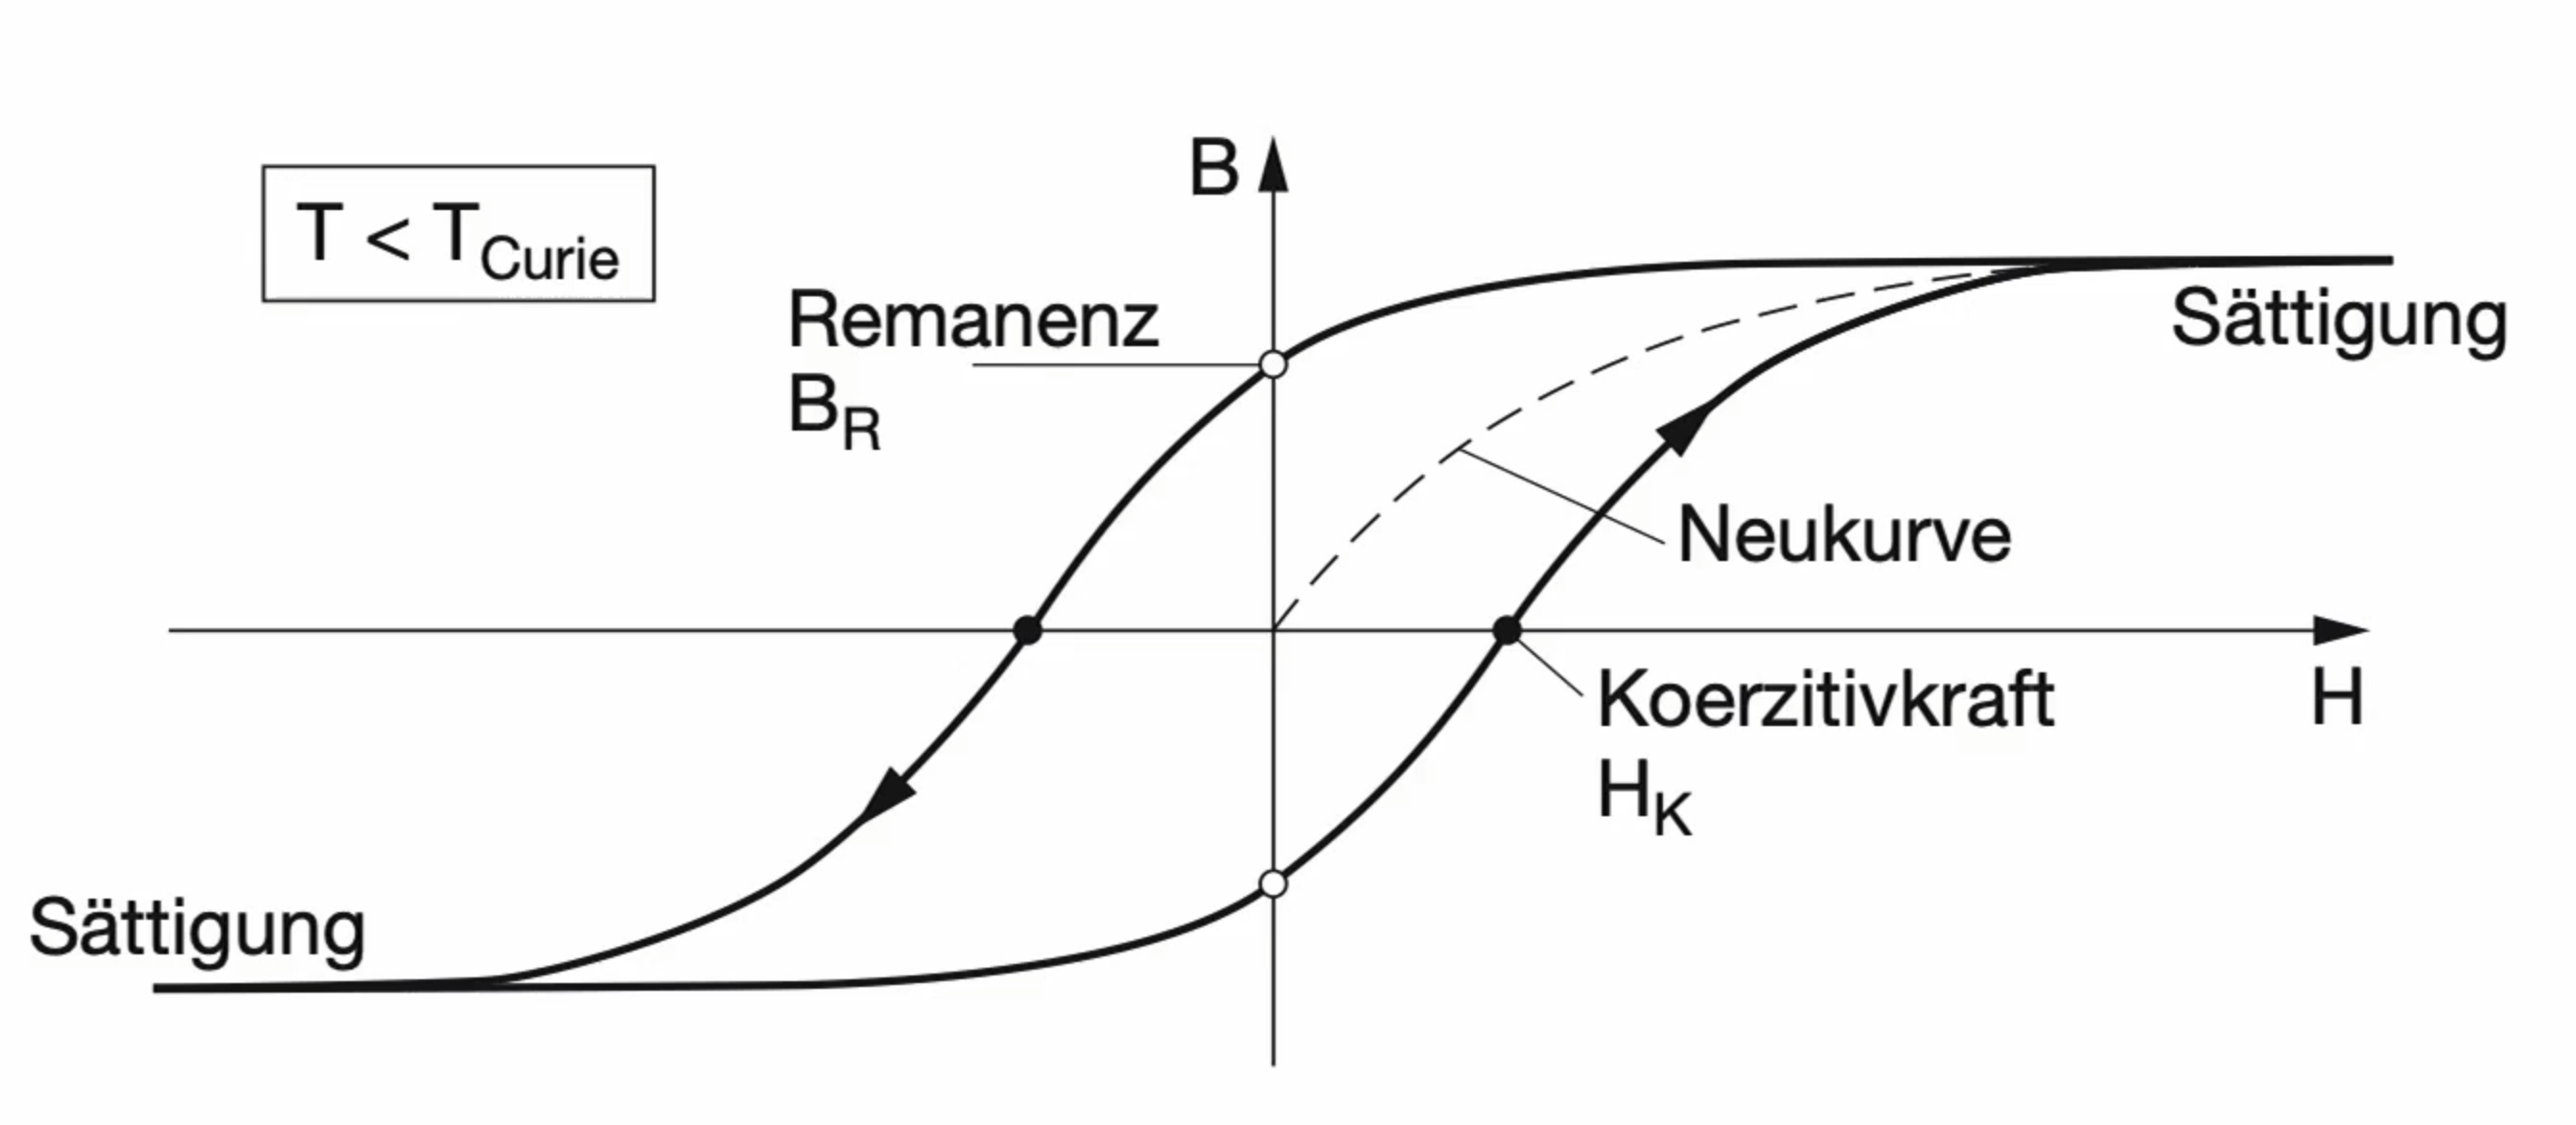
\includegraphics[width = \linewidth]{src/images/permanentmagnet.png}

    Meissner Effekt: Keine magnetischen Feldlinien treten in einen Supraleiter ein, perfektes diamagnetisches Verhalten.
    Anwendung: Magnet kann auf abgekühltem supraleiter-Material schweben, bsp. Magnetschwebebahn
    \subsection{Wechselspannung}
    \vspace{-1em}
    \begin{align*}
        \parbox{4cm}{\textbf{Komplexe Schreibweise:}}\\
        \overset{\sim}{I}(t) = I_0 e^{j \omega t}, \quad \overset{\sim}{U} &= \overset{\sim}{Z} \cdot \overset{\sim}{I} = I_0 Z \cdot e^{j \omega t} e^{j \rho}
        \\[0.5em]
        \parbox{4cm}{\textbf{Impedanz Spule:}}\\
        \overset{\sim}{Z}_S = R + j \omega L &= \sqrt{R^2 + \omega^2 L ^2} \cdot e^{j \rho}\\
        \text{Phasenverschiebung $\rho$:} \; U(t) &\sim I(t + \frac{\pi}{2})
        \\[0.5em]
        \parbox{4cm}{\textbf{Impedanz Kondensator:}}\\
        \overset{\sim}{Z}_C = - j\frac{1}{\omega C} &= \frac{1}{\omega C} \cdot e^{j \rho}\\
        \text{Phasenverschiebung $\rho$:} \; U(t) &\sim I(t - \frac{\pi}{2})
        \\[0.5em]
        \parbox{4cm}{\textbf{Impedanz Widerstand:}}\\
        \overset{\sim}{Z}_R = R &= R \cdot e^{j \rho}\\
        \text{Phasenverschiebung $\rho$:} \; U(t) &\sim I(t)
        \\[0.5em]
        \parbox{4cm}{\textbf{Leistung:}}\\
        P = \frac{1}{2} I_0 U_0 cos(\rho)\\
        \parbox{4cm}{\textbf{Winkel Phasenverschiebung im Schaltkreis:}}\\
        \tan(\Phi) = \frac{|Z_L| - |Z_C|}{Z_R}
    \end{align*}

    \tikzset{
        pattern size/.store in=\mcSize, 
        pattern size = 5pt,
        pattern thickness/.store in=\mcThickness, 
        pattern thickness = 0.3pt,
        pattern radius/.store in=\mcRadius, 
        pattern radius = 1pt}
        \makeatletter
        \pgfutil@ifundefined{pgf@pattern@name@_9395wxxuh}{
        \pgfdeclarepatternformonly[\mcThickness,\mcSize]{_9395wxxuh}
        {\pgfqpoint{-\mcThickness}{-\mcThickness}}
        {\pgfpoint{\mcSize}{\mcSize}}
        {\pgfpoint{\mcSize}{\mcSize}}
        {
        \pgfsetcolor{\tikz@pattern@color}
        \pgfsetlinewidth{\mcThickness}
        \pgfpathmoveto{\pgfpointorigin}
        \pgfpathlineto{\pgfpoint{0}{\mcSize}}
        \pgfusepath{stroke}
    }}
    \makeatother
    % Pattern Info
    \tikzset{
        pattern size/.store in=\mcSize, 
        pattern size = 5pt,
        pattern thickness/.store in=\mcThickness, 
        pattern thickness = 0.3pt,
        pattern radius/.store in=\mcRadius, 
        pattern radius = 1pt}
        \makeatletter
        \pgfutil@ifundefined{pgf@pattern@name@_r1aowurqw}{
        \pgfdeclarepatternformonly[\mcThickness,\mcSize]{_r1aowurqw}
        {\pgfqpoint{-\mcThickness}{-\mcThickness}}
        {\pgfpoint{\mcSize}{\mcSize}}
        {\pgfpoint{\mcSize}{\mcSize}}
        {
        \pgfsetcolor{\tikz@pattern@color}
        \pgfsetlinewidth{\mcThickness}
        \pgfpathmoveto{\pgfpointorigin}
        \pgfpathlineto{\pgfpoint{0}{\mcSize}}
        \pgfusepath{stroke}
    }}
    \makeatother
    \tikzset{every picture/.style={line width=0.75pt}} %set default line width to 0.75pt        

    \begin{center} 
        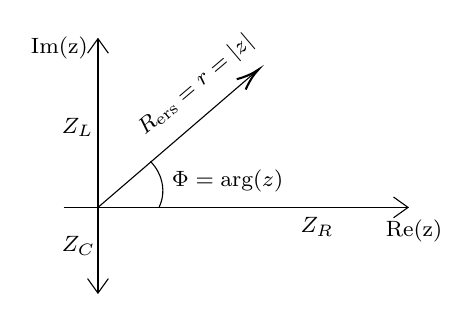
\begin{tikzpicture}[x=0.75pt,y=0.75pt,yscale=-1,xscale=1]
            %uncomment if require: \path (0,209); %set diagram left start at 0, and has height of 209
            % R_ers
            \draw (58.6,109.3) -- (134.1,44.4) ; % Line R_ers
            \draw [shift={(135.9,42.9)}, rotate = 139.32] [color={rgb, 255:red, 0; green, 0; blue, 0 }  ][line width=0.75]    (10.93,-3.29) .. controls (6.95,-1.4) and (3.31,-0.3) .. (0,0) .. controls (3.31,0.3) and (6.95,1.4) .. (10.93,3.29)   ; % Arrowhead R_ers
            \draw (74.22,68.61) node [anchor=north west][inner sep=0.75pt]  [font=\footnotesize,rotate=-319.68]  {$R_{\text{ers}} = r = |z|$}; % Text Node R_ers

            % Z_R
            \draw (42,109.3) -- (208,109.3); % Line Z_R
            \draw (201,104.3) -- (208,109.3) -- (201,114.3); % Arrowhead Z_R
            \draw (196,114) node [anchor=north west][inner sep=0.75pt]  [font=\footnotesize] [align=left] {Re(z)}; % Text Node Re(z)
            \draw (155,113) node [anchor=north west][inner sep=0.75pt]  [font=\footnotesize]  {$Z_R$}; % Text Node Z_R
            
            % Z_L
            \draw (58.6,28) -- (58.6,109.3); % Line Z_L
            \draw (53.6,35) -- (58.6,28) -- (63.6,35); % Arrowhead Z_L
            \draw (25,26) node [anchor=north west][inner sep=0.75pt]  [font=\footnotesize] [align=left] {Im(z)}; % Text Node Im(z)
            \draw (40,65) node [anchor=north west][inner sep=0.75pt]  [font=\footnotesize]  {$Z_L$}; % Text Node Z_L

            % Z_C
            \draw (58.6,109.3) -- (58.6,150.6); % Line Z_C
            \draw (53.6,143.6) -- (58.6,150.6) -- (63.6,143.6); % Arrowhead Z_C
            \draw (40,122) node [anchor=north west][inner sep=0.75pt]  [font=\footnotesize]  {$Z_C$}; %Text Node Z_C

            % Phi
            %\draw (83.87,147.15) .. controls (85.33,148.6) and (86.59,150.28) .. (87.58,152.18) .. controls (90.53,157.77) and (90.52,163.98) .. (88.13,169.06) -- (70.36,160.23) -- cycle ;
            \draw (83.87,87.15) .. controls (85.33,88.6) and (86.59,90.28) .. (87.58,92.18) .. controls (90.53,97.77) and (90.52,103.98) .. (88.13,109.06) ; % Angle Phi
            \draw (93,90) node [anchor=north west][inner sep=0.75pt]  [font=\footnotesize]  {$\Phi=\text{arg}(z)$};
        \end{tikzpicture}
    \end{center}

    % Spule: 
    % \mathbox{U_L = L \frac{dI}{dt}}

    % Kondensator:
    % \mathbox{U_C = \frac{1}{C} \int I(t) dt}

    % Impedanz:
    % \mathbox{Z_{\text{tot}} = \sum_i Z_i, \frac{1}{Z_{\text{tot}}} = \sum_i \frac{}{Z_i}}
    \vfill \null \columnbreak
    \subsection{Wechselstrom/Wechselspannung}    
    \begin{minipage}{0.49\linewidth}
        \centering \underline{\textbf{Gleichstrom}}\\
        \begin{empheq}[box = \fbox]{align*}
           I &= \frac{U}{R}
        \end{empheq}  
        \includegraphics*[width = \linewidth]{src/images/Gleichstrom.png}
    \end{minipage}
    \begin{minipage}{0.49\linewidth}
        \centering \underline{\textbf{Wechselstrom}}\\
        \begin{empheq}[box = \fbox]{align*}
            U &= U_0 \cdot \cos{\omega t}\\
            I &= \frac{U_0}{R}\cdot \cos{\omega t}
        \end{empheq} 
        \includegraphics*[width = \linewidth]{src/images/Wechselstrom.png}
    \end{minipage}

\subsection{Effektivwert}
    \begin{flushleft}
        Der Effektivwert ist jener Wert, der ein Gleichstrom haben müsste um die gleiche Leistung zu erzielen.\\      
    \end{flushleft}

    \begin{minipage}{0.49\linewidth}
        \centering \underline{\textbf{Sinus/Cosinuswellen}}\\
        \begin{empheq}[box = \fbox]{align*}
            P_\text{eff} &= \frac{1}{2} U_0 \cdot I_0\\
            \\
            U_\text{eff} &= \frac{1}{\sqrt{2}} \cdot U_0\\
            I_\text{eff} &= \frac{1}{\sqrt{2}} \cdot I_0
        \end{empheq} 
 
    \end{minipage}
    \begin{minipage}{0.49\linewidth}
        \centering \underline{\textbf{Allgemein}}\\
        \begin{empheq}[box = \fbox]{align*}
            P_\text{eff} &= \frac{1}{T} \int_{0}^{T}P dt \\
            \\
            U_\text{eff} &= \sqrt{\frac{1}{T} \int_{0}^{T} U^2 dt}
        \end{empheq} 
 
    \end{minipage}
    \includegraphics*[width = \linewidth]{src/images/Effektivwert.png}

\subsection{Wechselstrom und komplexe Zahlen}
    \begin{empheq}[box = \fbox]{align*}
        U(t) = U_0 \cos(\omega t+\varphi) &= U_0e^{j(\omega+\varphi)} &= U_0e^{j\omega} \cdot e^{\varphi}\\
        I(t) = I_0 \cos(\omega t+\varphi) &= I_0e^{j(\omega+\varphi)} &= I_0e^{j\omega} \cdot e^{\varphi}
    \end{empheq}

\subsection{Schein, Wirk und Blindleistung}
    \begin{minipage}{0.49\linewidth}
        \centering \underline{\textbf{Scheinleistung:}}\\
        \begin{empheq}[box = \fbox]{align*}
           S & = U_\text{eff} \cdot I_\text{eff}
        \end{empheq}
        \centering \underline{\textbf{Wirkleistung:}}\\
        \begin{empheq}[box = \fbox]{align*}
           P & = S \cdot \cos(\varphi)
        \end{empheq} 
        \centering \underline{\textbf{Blindleistung:}}\\
        \begin{empheq}[box = \fbox]{align*}
           Q & = S \cdot \sin(\varphi)
        \end{empheq}

    \end{minipage}
    \begin{minipage}{0.49\linewidth}
        \includegraphics*[width = \linewidth]{src/images/Scheinleistung.png}
        \includegraphics*[width = \linewidth]{src/images/Wirkleistung.png}


        \begin{empheq}[box = \fbox]{align*}
           S^2 = P^2 + Q^2
        \end{empheq} 

    \end{minipage}
    \vfill \null \columnbreak

\subsection{Impedanz/Blindwiderstände}
    \begin{minipage}{0.40\linewidth}
        \begin{empheq}[box = \fbox]{align*}
        U(t) &= U_0e^{j \omega t +\varphi_1}\\
        I(t) &= I_0e^{j \omega t +\varphi_2}
        \end{empheq} 
    \end{minipage}
    \begin{minipage}{0.58\linewidth}
        \begin{empheq}[box = \fbox]{align*}
        U &= R \cdot I\\
        U(t) &= Z \cdot I(t)
        \end{empheq} 
    \end{minipage}
    \begin{empheq}[box = \fbox]{align*}
        \text{Widerstand: } Z_R &= R\\
        \text{Kondensator: } Z_C &= -j\frac{1}{\omega C}\\
        \text{Spule: } Z_L &= j \omega L
    \end{empheq}

    \begin{minipage}{0.58\linewidth}
        \begin{empheq}[box = \fbox]{align*}
        U &= R \cdot I\\
        U(t) &= Z \cdot I(t)
        \end{empheq} 
    \end{minipage}
    
    \begin{minipage}{0.49\linewidth}
        \centering \underline{\textbf{Serie}}\\
        \includegraphics*[width=\linewidth]{src/images/Impedanz_Serie.png}
        \begin{empheq}[box = \fbox]{align*}
           Z &= R -j\frac{1}{\omega L} + j \omega L
        \end{empheq}  
    \end{minipage}
    \begin{minipage}{0.49\linewidth}
        \centering \underline{\textbf{Parallel}}\\
        \includegraphics*[width=\linewidth]{src/images/Impedanz_Parallel.png}
        \begin{empheq}[box = \fbox]{align*}
            \frac{1}{Z} &= \frac{1}{R} - \frac{1}{j\frac{1}{\omega L}} + \frac{1}{j \omega L}
        \end{empheq} 
    \end{minipage}
    \includegraphics*[width=\linewidth]{src/images/Wechselstrom_kompl.png}




\section{Elektromagnetische Wellen}
    \subsection{4.1 Herzscher Dipol}
    Elektrisches Pendel: Kondensator und Spule sind Energiespeicher.
    Wenn das magnetische Feld abgebaut wird, so wird das elektrische aufgebaut und umgekehrt.
    Idealisiert (ohne Reibung) "pendelt" dieses System unendlich lange
    \centering
    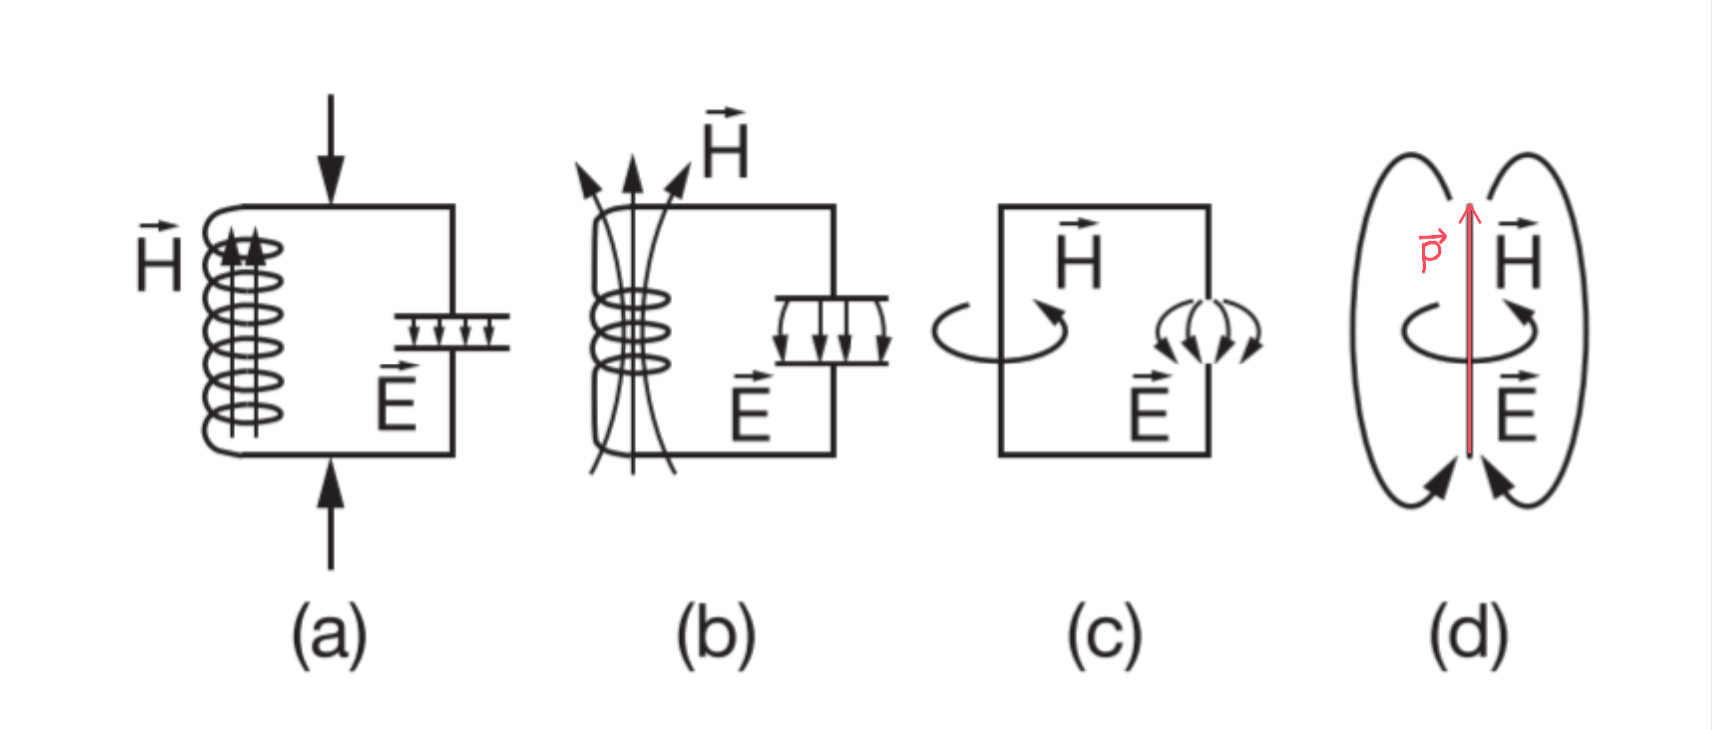
\includegraphics[height = 30mm]{src/images/herzscher_dipol.png}

    Dipolmoment $\vec{p}$ (alternierende Richtung durch Wechselspannung):
    \mathbox{\vec{p} = q \vec{l} = \vec{p_0} cos(\omega t)}

    Fernfeld: Entfernt man sich weit vom Sender (Herzschen Dipol), so verschwindet der phasenunterschied zwischen elektrischem und magnetischem Feld.

    \mathbox{\vec{E} = \vec{E_0} cos(\omega t - k r)}
    \mathbox{\vec{H} = \vec{H_0} cos(\omega t - k r)}
    mit Kreisfrequenz $\omega = 2 \pi \nu \rightarrow T = \frac{1}{\nu}$, Wellenzahl $k = \frac{2 \pi}{\lambda}$
    [$\nu = $ Frequenz, $T = $ Periode, $\lambda = $ Wellenlänge]
    \subsection*{4.2 Wellengleichung}
    \mathbox{\frac{\partial^2 E}{\partial t^2} = \frac{1}{\varepsilon_0 \mu_0} \frac{\partial^2 E}{\partial z^2}}
    \mathbox{\frac{\partial^2 H}{\partial t^2} = \frac{1}{\varepsilon_0 \mu_0} \frac{\partial^2 H}{\partial z^2}} 
    \subsection{4.3 Poynting-Vektor}
    Energiestromdichte und Poynting-Vektor:
    \mathbox{\vec{S} = \vec{E} \times \vec{H} = \vec{j_E}}

    Energiedichte:
    \mathbox{|\vec{j_E}| \approx \rho_E = \frac{1}{2} \varepsilon_0 E^2 + \frac{1}{2} \mu_0 H^2}
    \subsection*{4.4 Wellen}
    Höhe $\Phi$:
    \mathbox{\Phi (z, t) = A cos(\omega t - k z)}
    Wellenzahl $k = \frac{2 \pi}{\lambda}$, $z$ bezeichnet die entfernung zum Ursprung der cosinusfunktion zu Zeitpunkt $t_0$

    Phasengeschwindigkeit: Höhe konstant und somit Argument des cos() konstant:
    \mathbox{\omega t - k z = const}
    \mathbox{v_{ph} = c = f \lambda = \frac{\omega}{k}}
    Frequenz $f$

    Gruppengeschwindigkeit:
    \mathbox{v_{gr} = \frac{d \omega}{dk}}


    Intensität einer Welle: Energie
    Potentielle Energie:
    \mathbox{\Delta E_p = \int \overrightarrow{F} \overrightarrow{dx} = \frac{1}{2} D x_0^2 \text{mit} D = \omega^2 m}
    Kinetische Energie:
    \mathbox{\Delta E_k = \frac{1}{2} \Delta m v^2 \text{mit} v = \omega s}
    $\rightarrow \Delta E_p = \Delta E_k$  

    Energiestromdichte:
    \mathbox{\overrightarrow{j_E} = \frac{1}{A} \frac{\Delta E_k}{\Delta t} = \rho_E \overrightarrow{v_ph}}
    \subsection{Doppler-Effekt}
    \subsubsection{Ohne relativistischen Effekt (Bsp. Schall)}
    Wenn Empfänger sich auf Sender zubewegt:
    \mathbox{f' = f_0 (1 + \frac{v}{c})}

    \begin{minipage}{0.22\linewidth}
            \mathbox{\lambda_0 = \frac{c}{f_0}}
    \end{minipage}
    \begin{minipage}{0.70\linewidth}
        \begin{center}
            \begin{empheq}[box=\fbox]{align*}
                \text{Schallgeschwindigkeit: } &= 340 \frac{m}{s}\\
                \text{Lichtgeschwindigkeit: } &= 3 \cdot 10^8 \frac{m}{s}
            \end{empheq}
        \end{center}
    \end{minipage}
    \vspace{2mm}


    \begin{minipage}{0.49\linewidth}
        \textbf{Empfänger auf Sender:}\\
        \begin{center}
            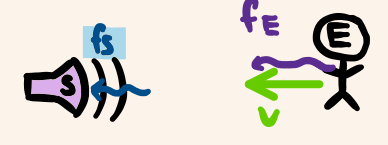
\includegraphics[width = 0.49\linewidth]{src/images/Doppler_E_zu_S.png}
        \end{center}
    \end{minipage}
    \begin{minipage}{0.49\linewidth}
        \begin{center}
            \begin{empheq}[box=\fbox]{align*}
                f' = f_0 (1 + \frac{v}{c})
            \end{empheq}
        \end{center}
    \end{minipage}
    \vspace{2mm}

    \begin{minipage}{0.49\linewidth}
        \textbf{Empfänger von Sender weg:}\\
        \begin{center}
            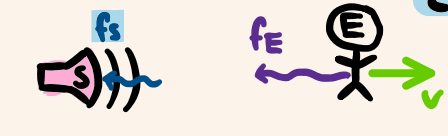
\includegraphics[width = 0.49\linewidth]{src/images/Doppler_E_weg_S.png}
        \end{center}
    \end{minipage}
    \begin{minipage}{0.49\linewidth}
        \begin{center}
            \begin{empheq}[box=\fbox]{align*}
                f' = f_0 (1 - \frac{v}{c})
            \end{empheq}
        \end{center}
    \end{minipage}
    \vspace{2mm}


    \begin{minipage}{0.49\linewidth}
        \textbf{Sender auf Empfänger:}\\
        \begin{center}
            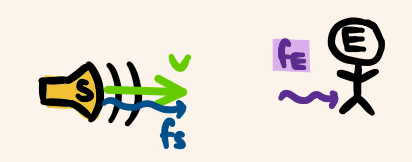
\includegraphics[width = 0.49\linewidth]{src/images/Doppler_S_zu_E.png}
        \end{center}
    \end{minipage}
    \begin{minipage}{0.49\linewidth}
        \begin{center}
            \begin{empheq}[box=\fbox]{align*}
                f' = f_0 \frac{1}{1 - \frac{v}{c}}
            \end{empheq}
        \end{center}
    \end{minipage}
    \vspace{2mm}


    \begin{minipage}{0.49\linewidth}
        \textbf{Sender von Empfänger weg:}\\
        \begin{center}
            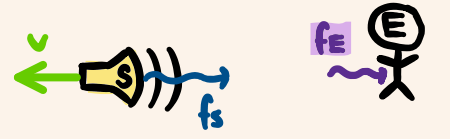
\includegraphics[width = 0.49\linewidth]{src/images/Doppler_S_weg_E.png}
        \end{center}
    \end{minipage}
    \begin{minipage}{0.49\linewidth}
        \begin{center}
            \begin{empheq}[box=\fbox]{align*}
                f' = f_0 \frac{1}{1 + \frac{v}{c}}
            \end{empheq}
        \end{center}
    \end{minipage}
    \vspace{2mm}

    \begin{flushleft}
    Für $v << c$ gilt, dass es nicht drauf ankommt ob Sender oder Empfänger sich in Ruhe befindet.

    \subsubsection{Mit relativistischem Effekt ($v \rightarrow c_0$)}
    $\beta = \frac{v}{c}$
    \vspace{2mm}

    
    
        \textbf{Quelle und Empfänger entfernen sich (Redshift):}\\
        \mathbox{f' = f_0 \sqrt{\frac{1 - \beta}{1 + \beta}}}

        \textbf{Quelle und Empfänger nähern sich (Blueshift):}\\
        \mathbox{f' = f_0 \sqrt{\frac{1 + \beta}{1 - \beta}}}
    \end{flushleft}\


    
    \newpage

\section{Appendix}
    \subsection*{5.1 LR-Kreise}
    LR-Kreise bestehen aus einer Gleichstromquelle, einem Schalter, einer Spule und einem Widerstand in Reihe geschalten.\\
    Maschenregel:
    \mathbox{U_0 = U_R(t) + U_L(t)}

    mit $U_R(t) = R I(t)$ und $U_L(t) = L \frac{dI(t)}{dt}$ und geteilt durch $L$
    DGL der Stromstärke und ihre Lösung:
    \mathbox{\dot{I}(t) + \frac{R}{L} I(t) = \frac{U_0}{L}, I(t) = \frac{U_0}{R} \left(1 - e^{-\frac{R}{L}t}\right)}
    \subsection{Energie/Kraftten}
\begin{flushleft}
    Energie:\\
    \begin{empheq}{align*}
        E_\text{pot} &= m \cdot h\\
        E_\text{kin} &= \frac{1}{2} m \cdot v^2\\
        E_\text{el} &= Q \cdot U\\
        E_\text{el,kond.} &= \frac{1}{2} \frac{Q^2}{C} = \frac{1}{2} C U^2 = \frac{1}{2} Q U = \frac{1}{2} \varepsilon_0 \frac{U^2}{d} A\\
        E_\text{el,spule} &= \frac{L \cdot I^2}{2}\\
        E_\text{photon} &= h \cdot f
    \end{empheq}

    Arbeit:\\
        \begin{empheq}{align*}
            W &= \int_{C} \vec{F} \vec{ds}\\
            W &= \int_{t_0}^{t_1} P(t) dt
        \end{empheq}

    Kraft:\\
    \begin{empheq}{align*}
        F &= m \cdot g\\
        F_\text{zptal} &= \frac{m \cdot v^2}{r}\\
        F_\text{g} &= m \cdot g\\
        F_\text{R} &= \mu \cdot F_\text{N}\\
        F_\text{Fed} &= R \cdot s\\
        F_\text{el,E-feld} &= Q \cdot E\\
        F_\text{el,Coul} &= \frac{1}{4\pi\varepsilon_0}\cdot \frac{q_1 \cdot q_2}
        {r^2}\cdot \vec{e_r}    
    \end{empheq}

    Weg/Geschwindigkeit/Beschleunigung:\\
    \begin{empheq}{align*}
        s &= [m]\\
        \frac{ds}{dt} &= \dot{s} = v = \frac{s}{t} = \left[\frac{m}{s}\right]\\
        \frac{ds^2}{dt^2} &= \ddot{s} = a =\frac{s}{t^2} = \left[\frac{m}{s^2}\right]\\
    \end{empheq}
\end{flushleft}

    
    \vfill \null \columnbreak

\section{Variabeln und Konstanten}
    \subsection{Variablen}
    \begin{empheq}{align*} % Dipolmoment???
        \vec{B}                              &\quad \text{Magnetische Induktion}             & \scriptstyle T = \frac{W b}{m^2} = \frac{V \cdot s}{m^2} = \frac{kg}{A \cdot s^2} \\
        C                                               &\quad \text{Kapazität}                         & \scriptstyle F = \frac{C}{V} = \frac{A \cdot s}{V} = \frac{A^2 \cdot s^4}{kg \cdot m^2} \\
        D                                               &\quad \text{elek. Flussdichte /}               & \scriptstyle \frac{A \cdot s}{m^2}\\
                                                        &\quad \text{Verschiebungsdichte}               & \\
        \vec{E}                              &\quad \text{e. Feld}                           & \scriptstyle \frac{N}{C} = \frac{V}{m} = \frac{kg \cdot m}{s^3 \cdot A} \\
        E                                               &\quad \text{Energie} \quad 1eV \cdot e = 1J    & \scriptstyle J = Nm = CV = Ws \frac{kg \cdot m^2}{s^2} \\
        \scriptstyle f = \nu = \frac{1}{T}              &\quad \text{Frequenz}                          & \scriptstyle \frac{1}{s} = Hz \\
        \vec{F}                              &\quad \text{Kraft}                             & \scriptstyle N = \frac{V \cdot C}{m} = \frac{kg \cdot m}{s^2} \\
        \vec{H}                              &\quad \text{magn. Feldstärke}                  & \scriptstyle \frac{A}{m} \\
        \vec{I}                              &\quad \text{el. Strom}                         & \scriptstyle A = \frac{C}{s} \\
        \scriptstyle \vec{j} = \frac{I}{A}   &\quad \text{Stromdichte}                       & \scriptstyle \frac{C}{s \cdot m^2} \\
        k                                               &\quad \text{Federkonstante}                    & \scriptstyle \frac{N}{m} \\
        L                                               &\quad \text{Induktivität}                      & \scriptstyle H = \frac{T \cdot m^2}{A} = \frac{V \cdot s}{A} \\
                                                        &                                               & \scriptstyle = \frac{kg \cdot m^2}{A^2 \cdot s^2} \\
        P                                               &\quad \text{Leistung}                          & \scriptstyle W = V \cdot A = \frac{J}{s} \\
        Q                                               &\quad \text{Ladung}                            & \scriptstyle C = A \cdot s \\
        R                                               &\quad \text{el. Widerstand}                    & \scriptstyle \Omega = \frac{V}{A} \\
        S                                               &\quad \text{Siemens}                           & \scriptstyle S = \frac{1}{\Omega} = \frac{A}{V} \\
        T                                               &\quad \text{Periodendauer /}                   & \scriptstyle s \\
                                                        &\quad \text{Schwingungsdauer}                  & \\
        U                                               &\quad \text{Potentialdiff. / Spannung}         & \scriptstyle V = \frac{W}{A} = \frac{J}{C} \\
                                                        &                                               & \scriptstyle = \frac{Nm}{As} = \frac{kg \cdot m^2}{A \cdot s^3} \\
        \vec{v}                              &\quad \text{Geschwindigkeit}                   & \scriptstyle \frac{m}{s} \\
        W                                               &\quad \text{Arbeit}                            & \scriptstyle J = N \cdot m \\
                                                        &                                               & \scriptstyle = \frac{kg \cdot m^2}{s^2} = C \cdot V \\
        Z                                               &\quad \text{Impedanz}                          & \scriptstyle \Omega = \frac{V}{A} = \frac{kg \cdot m^2}{A^2 \cdot s^3} \\
        \varepsilon                                     &\quad \text{Dielektrizitätskonst. Mat.}        & \scriptstyle \frac{C}{V \cdot m} = \frac{A \cdot s}{V \cdot m} \\
        \Psi_E                                          &\quad \text{elek. Fluss}                       & \scriptstyle V \cdot m = \frac{N \cdot m^2}{C} \\
        \Phi_M                                          &\quad \text{magn. Fluss}                       & \scriptstyle Wb = T \cdot m^2 \\
        \Phi                                            &\quad \text{elek. Potential}                   & \scriptstyle [-] \\
        \lambda = \frac{c}{f}                           &\quad \text{Wellenlänge}                       & \scriptstyle m \\
        \mu                                             &\quad \text{magn. Feldk. /}                    & \scriptstyle \frac{V \cdot s}{A \cdot m} \\
                                                        &\quad \text{Permeabilität}                     & \\
        \rho                                            &\quad \text{spez. Widerstand}                  & \scriptstyle \Omega \cdot m \\
        \omega = 2 \pi f                                &\quad \text{Kreisfrequenz}                     & \scriptstyle s^{-1} = Hz \\
        %&\quad \text{} & \scriptstyle  \\
    \end{empheq}
    \subsection{Einheiten}
    \begin{empheq}{align*}
        eV                                              &\quad \text{Elektronenvolt (Energie)}          & \scriptstyle 1 e \cdot 1 V  \approx 1.6 \cdot 10^{-19} J\\
        u                                               &\quad \text{Atomare Masseneinheit}             & \scriptstyle 1,66054 \cdot 10^{-27} kg \\
        1 \frac{m}{s}                                   &\quad \xrightarrow{\cdot 3.6} 1 \frac{km}{h}   & \\
    \end{empheq}
    \vfill \null \columnbreak

    \subsubsection{Konstanten}
    \begin{empheq}{align*}
        g                                               &\quad \text{Fallbeschleunigung}                & \scriptstyle g \approx 9.81 \frac{m}{s^2} = \frac{N}{kg}\\
        \varepsilon_0                                   &\quad \text{el. Feldkonst /}                   & \scriptstyle \varepsilon_0 = \frac{1}{\mu_0 \cdot c_0^2} = \frac{10^7}{4 \pi c_0^2}\\
                                                        &\quad \text{Dielektrizitätskonst. /}           & \\
                                                        &\quad \text{Permittivität Vakuum}              & \\
        \varepsilon_{r, vak}                            &\quad \text{Permittivitätszahl Vakuum}         & \scriptstyle \varepsilon_{r, vak} = 1\\
        c_0                                             &\quad \text{Lichtgesch. Vakuum}                & \scriptstyle \frac{1}{\sqrt{\varepsilon_0 \mu_0}} \approx 3 \cdot 10^8 \frac{m}{s} \\
        \mu_0                                           &\quad \text{magn. Feldk. /}                    & \scriptstyle \mu_0 = \frac{1}{\varepsilon_0 c_0^2} = 4 \pi \cdot 10^{-7} \frac{V \cdot s}{A \cdot m} \\
                                                        &\quad \text{Permeabilität Vakuum}              & \\
        \mu_{r, vak}                                     &\quad \text{Permeabilitätszahl Vakuum}         & \scriptstyle \mu_{r, vak} = 1\\
        e                                               &\quad \text{Elementarladung}                   & \scriptstyle 1,602 \cdot 10^{-19} C \\
        m_e                                             &\quad \text{Elektronenmasse}                   & \scriptstyle = 9,11 \cdot 10^{-31} kg \\
        &\quad \text{} & \scriptstyle  \\
    \end{empheq}

    \subsection{Nutzliche Formeln}
    \begin{empheq}{align*}
        F_Z                                             &\quad \text{Zentripetalkraft}                  & \scriptstyle = m \frac{v^2}{r} = m \omega^2 r \\
        |\vec{a} \times \vec{b}|  &\quad \text{Kreuzprodukt}                      & \scriptstyle = |\vec{a}| \cdot |\vec{b}| \cdot \sin(\alpha)
    \end{empheq}

    \subsubsection{Rechengesetze für Exponenten \& Logarithmen}
        \begin{minipage}{0.29\linewidth}
            \begin{empheq}{align*}
                B^a \cdot B^b =& \; B^{a + b}\\
                \frac{B^a}{B^b} =& \; B^{a - b}\\
                (B^a)^b =& \; B^{a \cdot b}
            \end{empheq}
        \end{minipage}
        \begin{minipage}{0.69\linewidth}
            \begin{empheq}{align*}
                \log_B (a \cdot b ) =& \; \log_B (a) + \log_B (b)\\
                \log_B \left( \frac{a}{b} \right) =& \; \log_B (a) - \log_B (b)\\
                \log_B (a^r) =& \; r \cdot \log_B (a)
            \end{empheq}
        \end{minipage}
        \begin{align*}
            \textrm{Basiswechsel: } \log_a (x) =& \; \frac{\log_b(x)}{\log_b(a)}
        \end{align*}

    \subsection{Vorsilben und Exponente}
    \begin{tabular}{c c c c c c c}
        \textbf{Symbol}     & P         & T         & G         & M         & k         & h   \\
        \textbf{Silbe}      & Peta      & Terra     & Giga      & Mega      & kilo      & hekto \\
        \textbf{Exponent}   & $10^{15}$ & $10^{12}$ & $10^9$    & $10^6$    & $10^3$    & $10^2$
    \end{tabular}
    \begin{tabular}{c c c c c c c c}
        d         & c         & m         & $\mu$         & n         & p           & f \\
        deci      & centi     & milli     & micro         & nano      & pico        & femto \\
        $10^{-1}$ & $10^{-2}$ & $10^{-3}$ & $10^{-6}$     & $10^{-9}$ & $10^{-12}$  & $10^{-15}$
    \end{tabular}
%        Y & $10^{24}$ \\
%        Z & $10^{21}$ \\
%        E & $10^{18}$ \\
%        da & $10^1$ \\
%        a & $10^{-18}$ \\
%        z & $10^{-21}$ \\
%        y & $10^{-24}$ 
    \newpage

\section{Beispiele}
    \subsection{Beispiele Elektrisches Feld}
    \subsubsection{Punktladung}
        \begin{minipage}{0.41\linewidth}
            \begin{footnotesize}
                \begin{center}
                    \vspace{2mm}
                    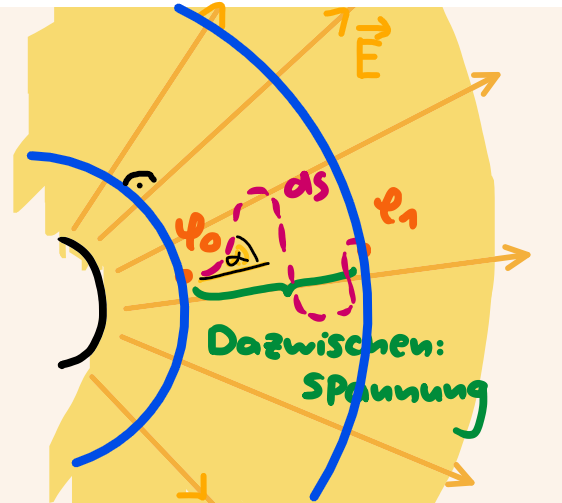
\includegraphics[width = 25mm]{src/images/inhom_potentialfeld.png}
                \end{center}
            \end{footnotesize}
        \end{minipage}
        \begin{minipage}{0.58\linewidth}
            \begin{scriptsize}
                \begin{center}
                    \begin{empheq}[box = \fbox]{align*}
                    %\mathbox{
                        U &= \int_{1}^{2}E\cdot\cos (\alpha) ds\\
                        &= \int_{1}^{2}\vec{E}(r)\:\vec{dr}
                    \end{empheq}
                    Auf \colorbox{Cyan}{Kreis $\Phi_{0/1}$} stets selbes Potential/Spannung
                \end{center}
            \end{scriptsize}
        \end{minipage}

    \subsubsection{Spannungswaage / Thompson-Waage}
        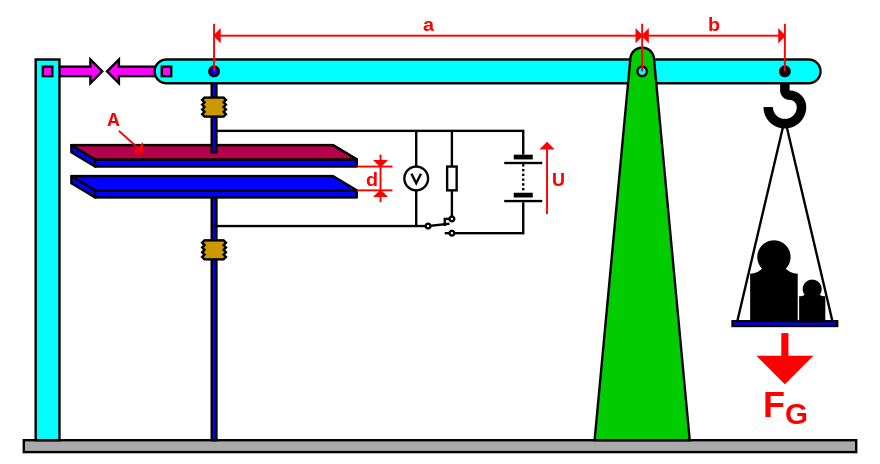
\includegraphics[width = 0.99\linewidth]{src/images/spannungswaage.png}
        \begin{minipage}{0.63\linewidth}
            \centering
            Kräftegleichgewicht:
            \begin{empheq}[box = \fbox]{align*}
                F_E &= \frac{E \cdot Q}{2} = \frac{1}{2} \varepsilon_0 \varepsilon_r \frac{A}{d^2} U^2\\
                F_G &= m \cdot g\\
                a \cdot F_E &= b \cdot F_G
            \end{empheq}
        \end{minipage}
        \begin{minipage}{0.35\linewidth}
            \begin{scriptsize}
                \begin{empheq}{align*}
                    F_E &= \text{elektrostatische Kraft}\\
                    F_G &= \text{Gewichtskraft}\\
                    m &= \text{Masse} [kg]\\
                    g &= \text{Fallbeschleunigung}\\
                    E &= \text{Elektrische Feldstärke}\\
                    Q &= \text{Ladungsmenge}\\
                    \varepsilon_r &= \text{Permittivität}
                \end{empheq}
            \end{scriptsize}
        \end{minipage}


    \subsubsection{Elektrisches Feld Kugel / Punktladung}
        \begin{minipage}{0.59\linewidth}
            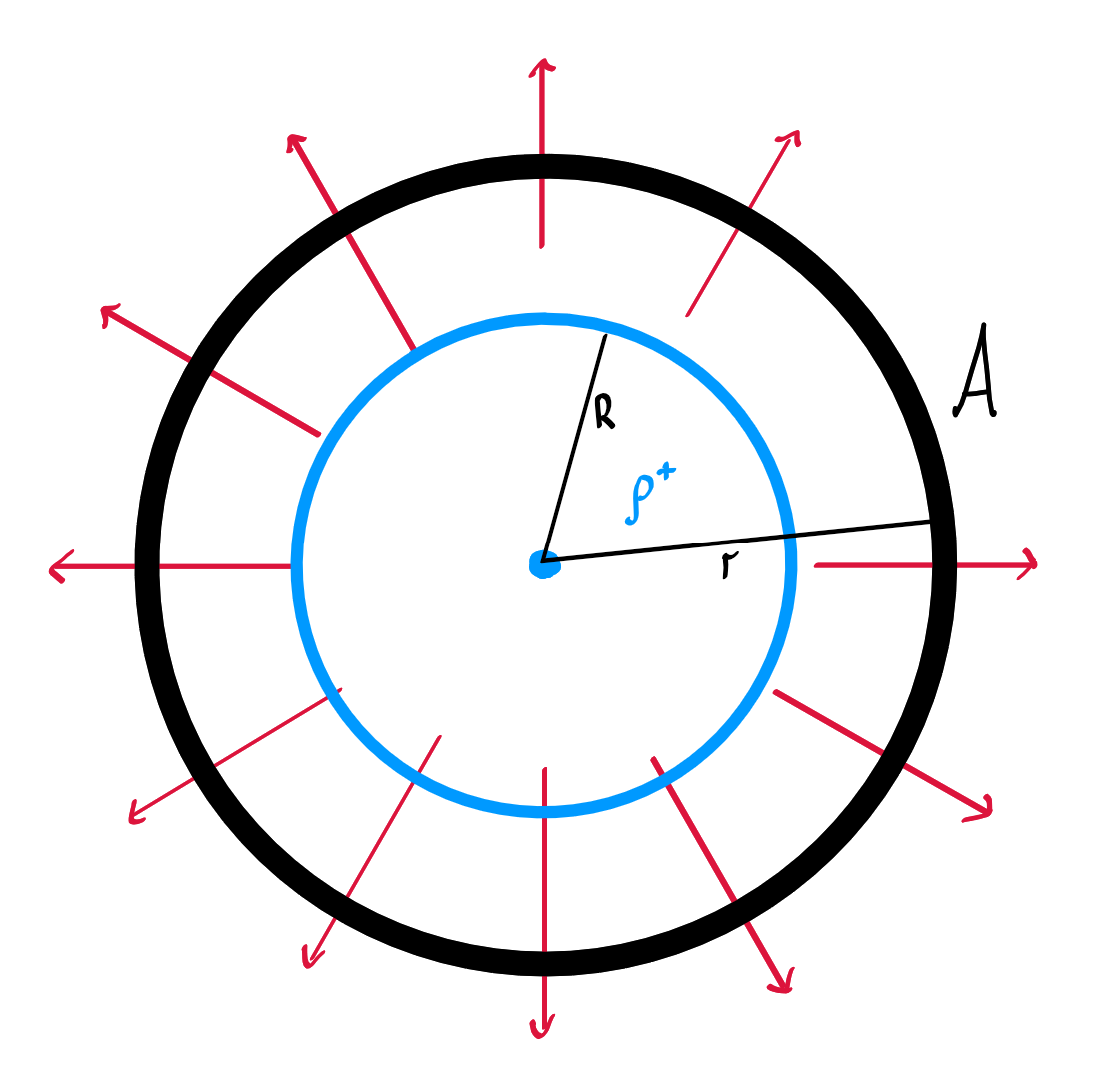
\includegraphics[width = \linewidth]{src/images/e-feld_punktladung.png}
        \end{minipage}
        \begin{minipage}{0.39\linewidth}
            \begin{empheq}{align*}
                \oint \vec{E} \vec{dA} &= \frac{1}{\varepsilon_0} \int \rho dV\\
                \rho&= \frac{Q}{V} = \frac{3Q}{4 \pi R^3}
            \end{empheq}
        \end{minipage}
        \[\begin{array}{c | c}
            r < R & r \geq R\\
            \hline \hline
            \Rightarrow E \cdot 4 \pi r^2 = \frac{\rho \cdot \frac{4}{3} \pi r^3}{\varepsilon_0} & \Rightarrow E \cdot 4 \pi r^2 = \frac{\rho \cdot \frac{4}{3}\pi R^3}{\varepsilon_0}\\
            \Rightarrow E = \frac{\rho r}{3 \varepsilon_0} = \frac{1}{4 \varepsilon_0 \pi } \frac{Q r}{R^3} & \Rightarrow E = \frac{\rho R^3}{3 \varepsilon_0 r^2} = \frac{1}{4 \varepsilon_0 \pi} \frac{Q}{r^2}
        \end{array}\]

    \vfill \null \columnbreak

    \subsubsection{Elektrisches Feld gerader Leiter}
        \begin{minipage}{0.39\linewidth}
            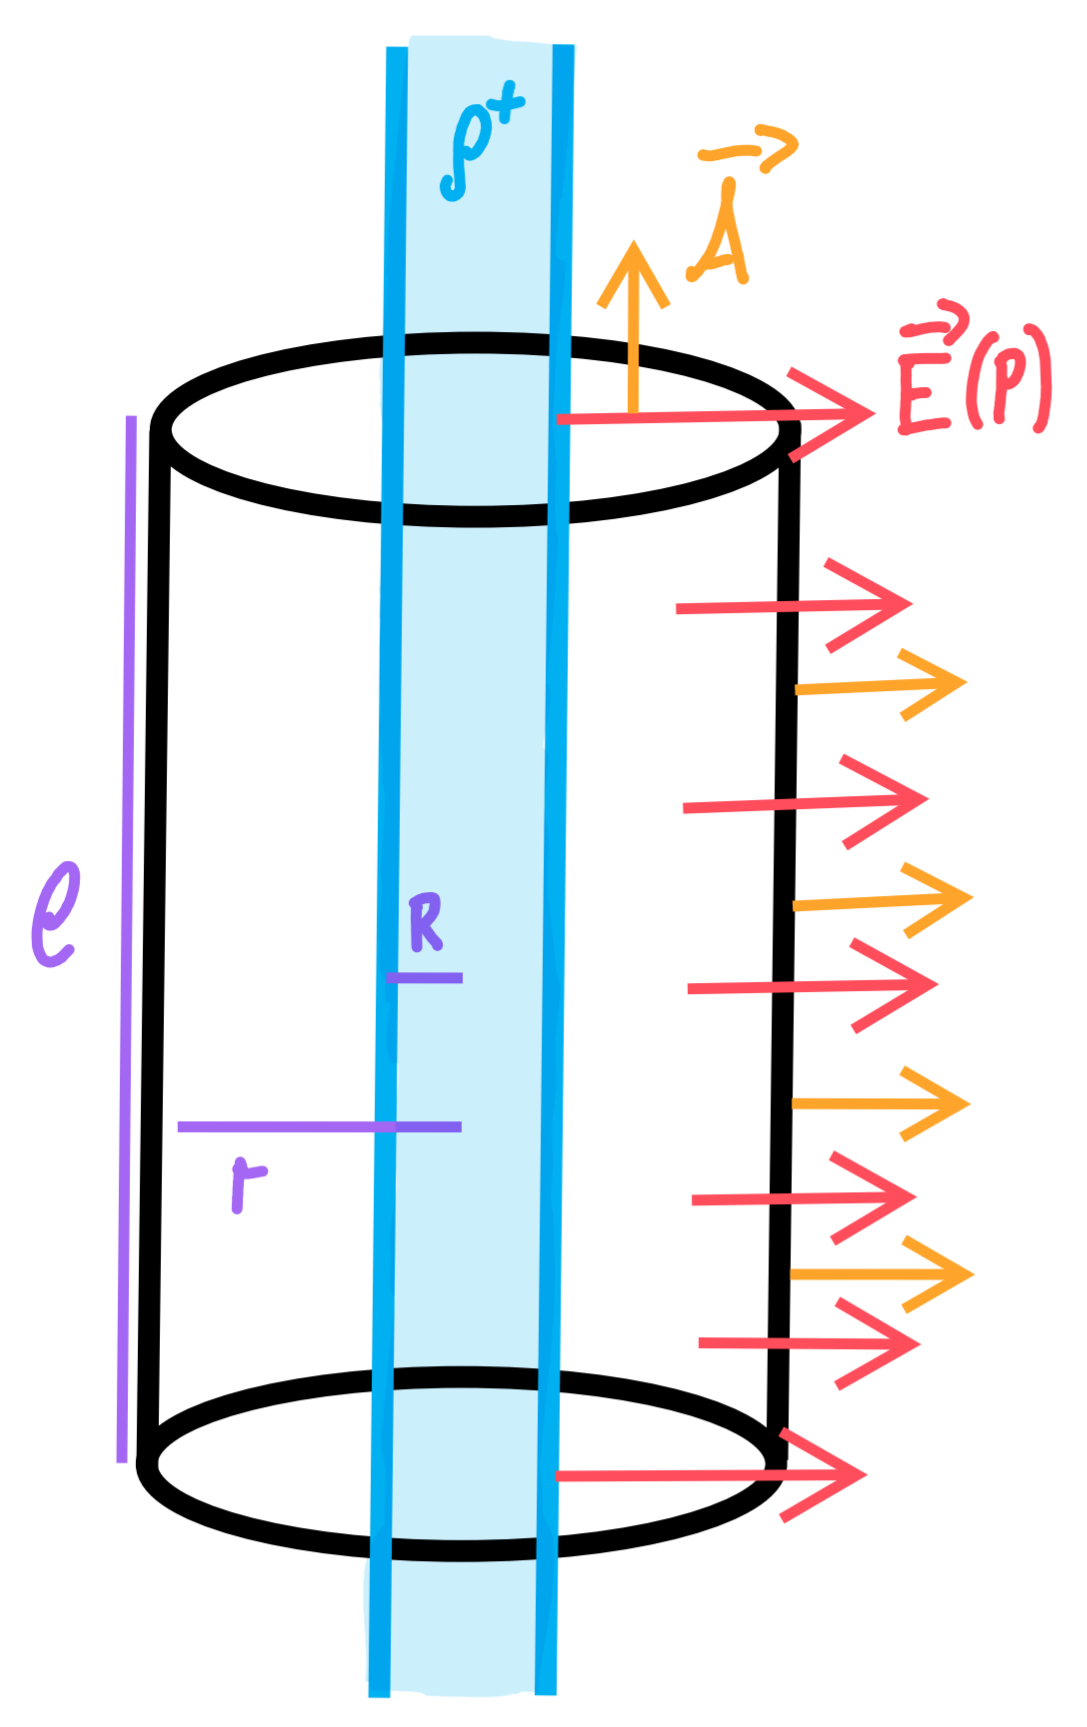
\includegraphics[width = \linewidth]{src/images/e-feld_gerader_leiter.png}
        \end{minipage}
        \begin{minipage}{0.59\linewidth}
            \begin{empheq}{align*}
                \oint \vec{E} \vec{dA} &= \frac{1}{\varepsilon_0} \int \rho dV\\
                \rho &= \frac{Q}{V} = \frac{3Q}{4 \pi R^3}\\
            \end{empheq}
        \end{minipage}
        \[\begin{array}{c | c}
            r < R & r \geq R\\
            \hline \hline
            E \cdot 2 \pi r \cdot l = \frac{\rho}{\varepsilon_0} \pi r^2 l & E \cdot 2 \pi r \cdot l = \frac{\rho}{\varepsilon_0} \pi R^2 l\\
            E = \frac{\rho}{2 \varepsilon_0} r & E = \frac{\rho}{2 \varepsilon_0} \frac{R^2}{r}
        \end{array}\]

    \subsubsection{Elektrisches Feld Platte}
        \begin{minipage}{0.49\linewidth}
            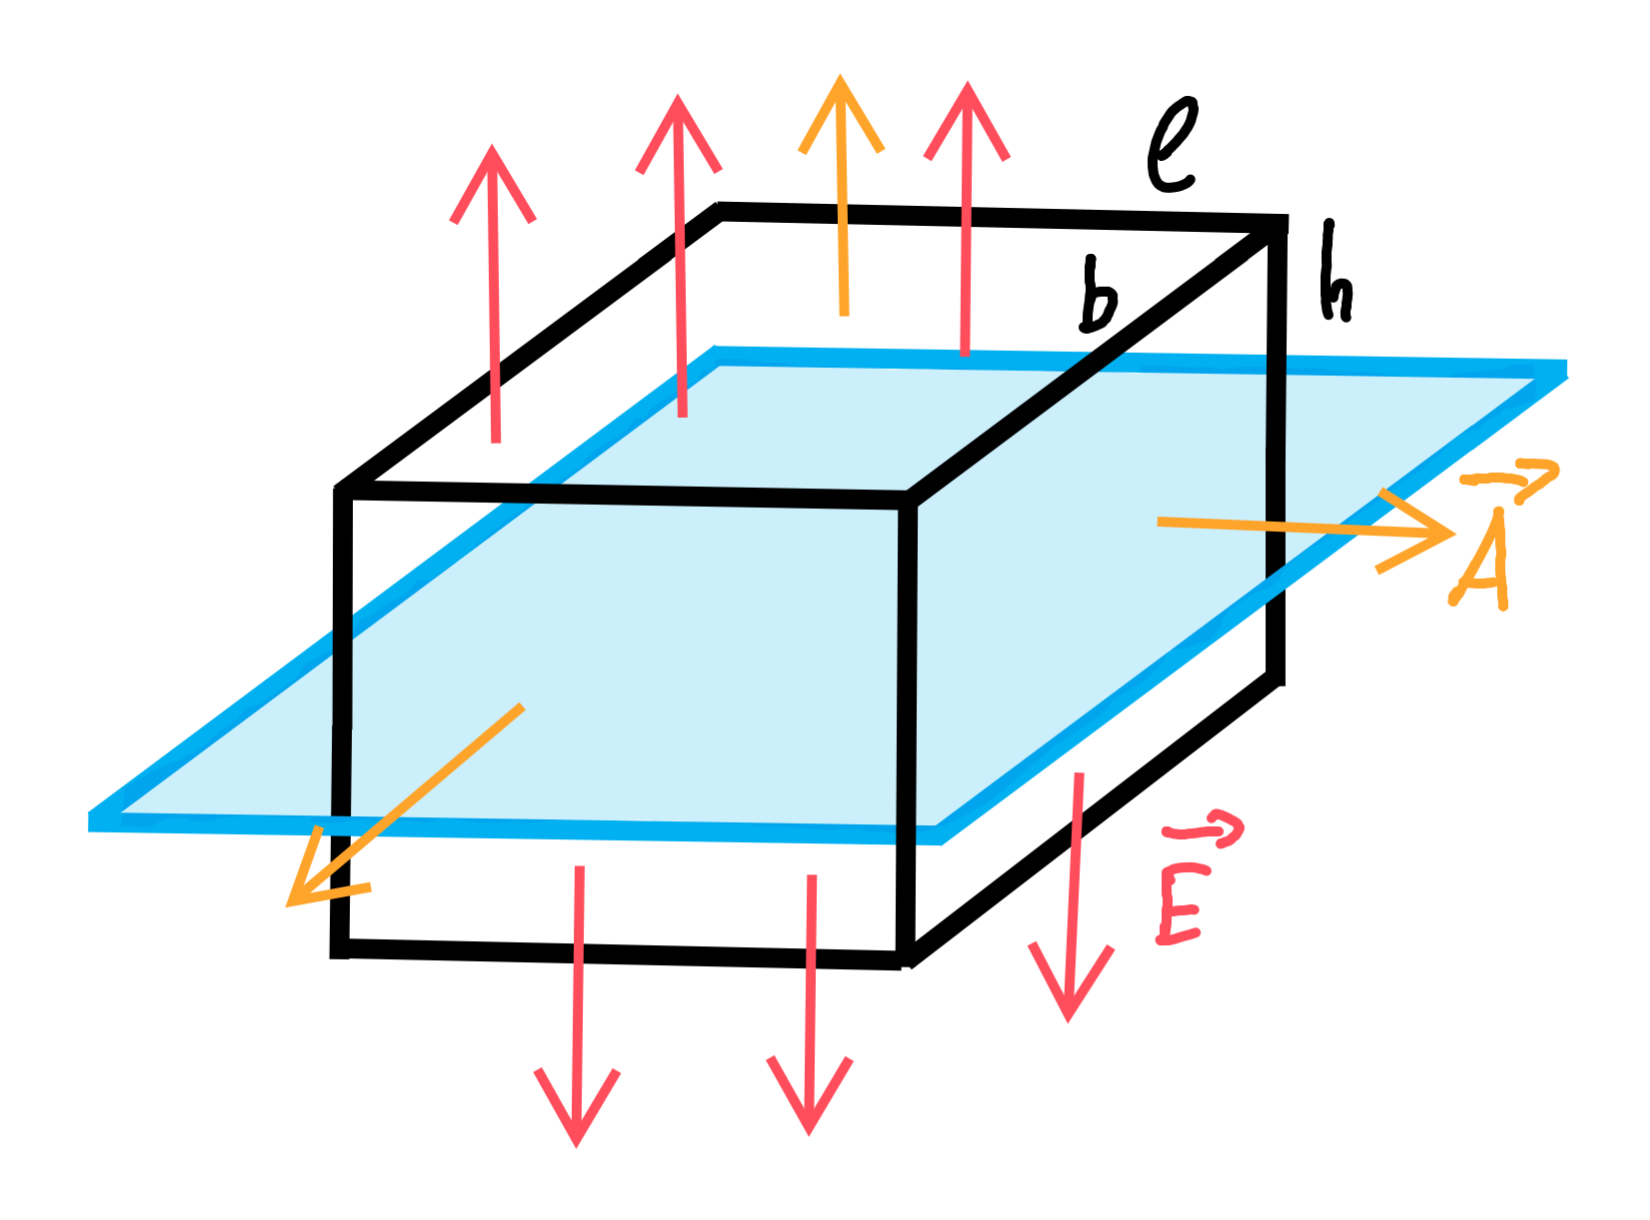
\includegraphics[width = \linewidth]{src/images/e-feld_platte.png}
        \end{minipage}
        \begin{minipage}{0.49\linewidth}
            \begin{empheq}{align*}
                &\oint \vec{E} \vec{dA} = \frac{1}{\varepsilon_0} \int \rho dV\\
                &\rho = \frac{Q}{A} = \frac{Q}{l \cdot b}\\
                \Rightarrow &E \cdot 2 l \cdot b = \frac{1}{\varepsilon_0} l \cdot \rho\\
                \Aboxed{\Rightarrow &E = \frac{\rho}{2 \varepsilon_0}}
            \end{empheq}
        \end{minipage}

    \subsubsection{Arten von Kondensatoren}
        {\centering \underline{\textbf{Plattenkondensator}} \par}
        \begin{minipage}{0.49\linewidth}
            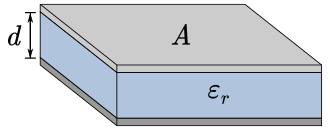
\includegraphics[width = \linewidth]{src/images/plattenkond.png}
        \end{minipage}
        \begin{minipage}{0.49\linewidth}
            \begin{empheq}[box=\fbox]{align*}
                C &= \varepsilon_0 \cdot \varepsilon_r \frac{A}{d}
            \end{empheq}
        \end{minipage}
        
        {\centering \underline{\textbf{Zylinderkondensator}} \par}
        \begin{minipage}{0.49\linewidth}
            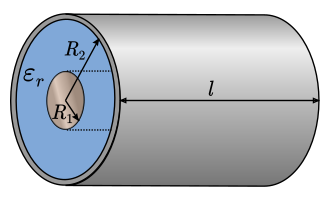
\includegraphics[width = \linewidth]{src/images/zylinderkond.png}
        \end{minipage}
        \begin{minipage}{0.49\linewidth}
            \begin{empheq}[box=\fbox]{align*}
                C &= 2\pi \varepsilon_0\cdot \varepsilon_r \frac{l}{\ln(\frac{r_2}{r_1})}
            \end{empheq}
        \end{minipage}
        
        {\centering \underline{\textbf{Kugelkondensator}} \par}
            \begin{minipage}{0.39\linewidth}
                {\centering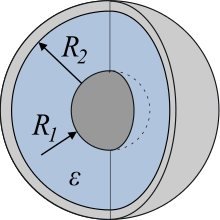
\includegraphics[width = 0.9\linewidth]{src/images/kugelkondensator.png} \par}
            \end{minipage}
            \begin{minipage}{0.59\linewidth}
                \begin{empheq}[box=\fbox]{align*}
                    C &= 4 \pi \varepsilon_0 \cdot \varepsilon_r \left(\frac{r_1 \cdot r_2}{r_2 - r_1}\right)
                \end{empheq}
            \end{minipage}

            Herleitung Kugelkondensator:\\
            \begin{empheq}{align*}
                C &= \frac{Q}{U}\\
                U &= \int_{r_1}^{r_2} \vec{E}(r) d \vec{r}\\
                E(r) &= \frac{D(r)}{\varepsilon_0 \varepsilon_r} = \frac{Q}{\varepsilon_0 \varepsilon_r A} = \frac{Q}{4 \pi \varepsilon_0 \varepsilon_r r^2}
            \end{empheq}
    \vfill \null \columnbreak
    \subsection{Beispiele Magnetisches Feld}
    \subsubsection{Leiterschleife mit verschiebbarem Bügel}
        ACHTUNG: Richtung der eingeführten Vektoren im Rechtssystem\\
        $\vec{l}$ in Richtung des Elektronenflusses
        \includegraphics[width = \linewidth]{src/images/leiterschleife_bügel_verschiebbar.png}
        \mathbox{d\vec{A} = d\vec{s} \times \vec{l} \rightarrow \frac{d \vec{A}}{dt} = \vec{v} \times \vec{l}}
        Induktionsgesetz:
        \begin{empheq}[box = \fbox]{align*}
            U_i &= -\frac{d}{dt} \int \vec{B} d\vec{A} = -\frac{d}{dt} \left( \vec{B} \vec{A} \right)\\
            &= \left(\vec{v} \times \vec{B} \right) \vec{l} - \vec{A} \frac{d \vec{B}}{dt}
        \end{empheq}

    \subsubsection{Feldstärke eines geradlinigen Leiters}
        \begin{minipage}{0.34\linewidth}
            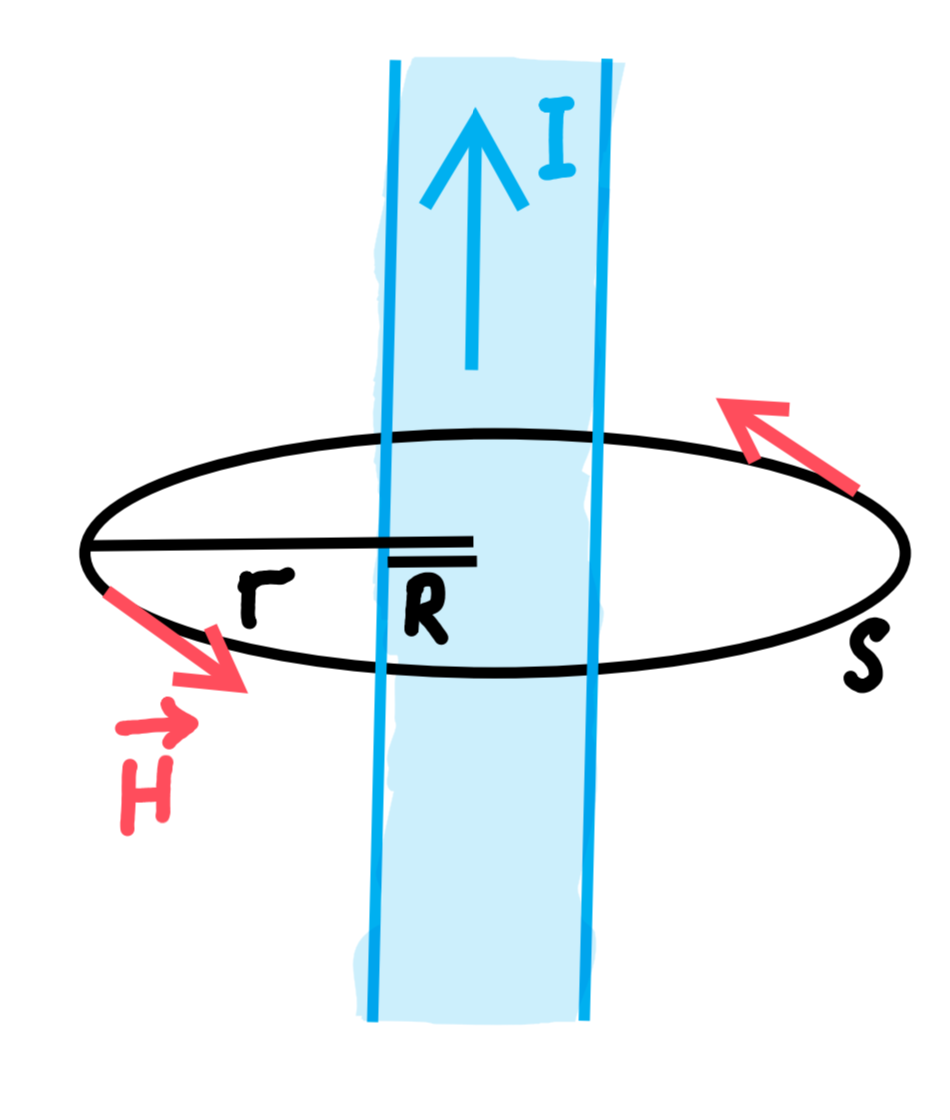
\includegraphics[width = \linewidth]{src/images/mag-feld_gerader_leiter.png}
        \end{minipage}
        \begin{minipage}{0.64\linewidth}
            Durchflutungsgesetz führt zu:
            \begin{empheq}[box = \fbox]{align*}
                \text{In Leiter: } H(r) &= \frac{I}{2 \pi} \frac{r}{R^2}\\
                \text{Um Leiter: } H(r) &= \frac{I}{2 \pi r}
            \end{empheq}
            \begin{scriptsize}
                \begin{empheq}{align*}
                    H &= \text{mag. Feldstärke}\\
                    I &= \text{el. Strom}\\
                    R &= \text{Radius des el. Leiters}\\
                \end{empheq}
            \end{scriptsize}
        \end{minipage}
    
    \subsubsection{Magnetfeld gerader Draht}
        {\centering Aus \ref{sec_biot_savart} Biot-Savart Gesetz \par}
            \begin{minipage}{0.39\linewidth}
                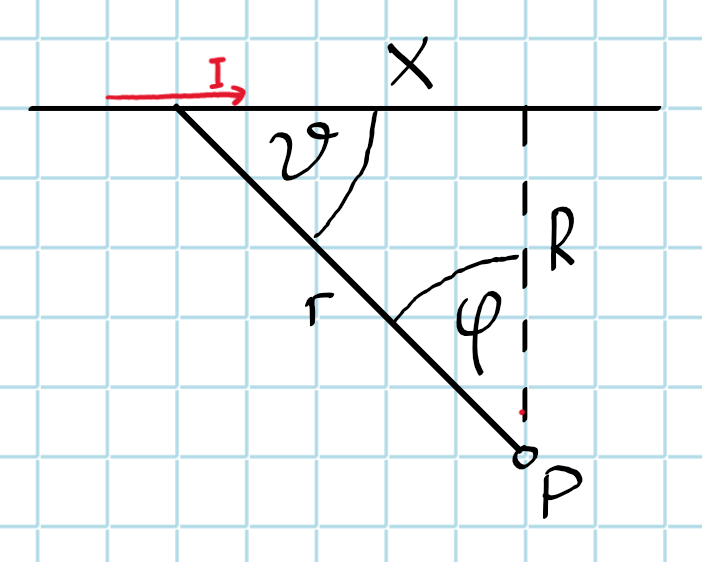
\includegraphics[width = \linewidth]{src/images/magnetfeld_draht.png}
            \end{minipage}
            \begin{minipage}{0.59\linewidth}
                \begin{empheq}[box = \fbox]{align*}
                    \vec{B} &= \frac{\mu_0}{4 \pi} I \int\limits_{-\infty}^{+\infty} \frac{dx \cdot |\hat{r}| \cdot \sin{\vartheta}}{r^2}\\
                    &= \frac{\mu_0}{4 \pi} I \int\limits_{-\frac{\pi}{2}}^{+\frac{\pi}{2}} \frac{\cos{\varphi}}{R} d\varphi
                \end{empheq}
            \end{minipage}
            \begin{scriptsize}
                \begin{align*}
                    \sin(\vartheta) = \frac{R}{r} = \cos(\varphi) \quad &\mid \quad r = \frac{R}{\cos(\varphi)}\\
                    x = R \tan(\varphi) \quad &\mid \quad dx = \frac{R}{\cos^2(\varphi)} d\varphi
                \end{align*}
            \end{scriptsize}
    
    \vfill \null \columnbreak

    \subsubsection{Beispiel Elektromotor}
        \begin{minipage}{0.54\linewidth}
            \begin{empheq}[box = \fbox]{align*}
                M &= I (\vec{A} \times \vec{B})\\
                M_{\text{dip}} &= \vec{m} \times \vec{B}\\
                W &= -\int M_{\text{dip}} d\alpha = \vec{m} \vec{B}
            \end{empheq}
            \begin{scriptsize}
                \begin{empheq}{align*}
                    \vec{A} &= \text{Vektor normal zu Fläche}\\
                    \vec{B} &= \text{mag. Flussdichte}\\
                    \vec{m} &= \text{mag. Dipolmoment}\\
                \end{empheq}
            \end{scriptsize}
        \end{minipage}
        \begin{minipage}{0.44\linewidth}
            "Kommutator" kehrt Polarisierung des Stroms nach halber Umdrehungen um, damit volle Umdrehung ermöglicht wird.
            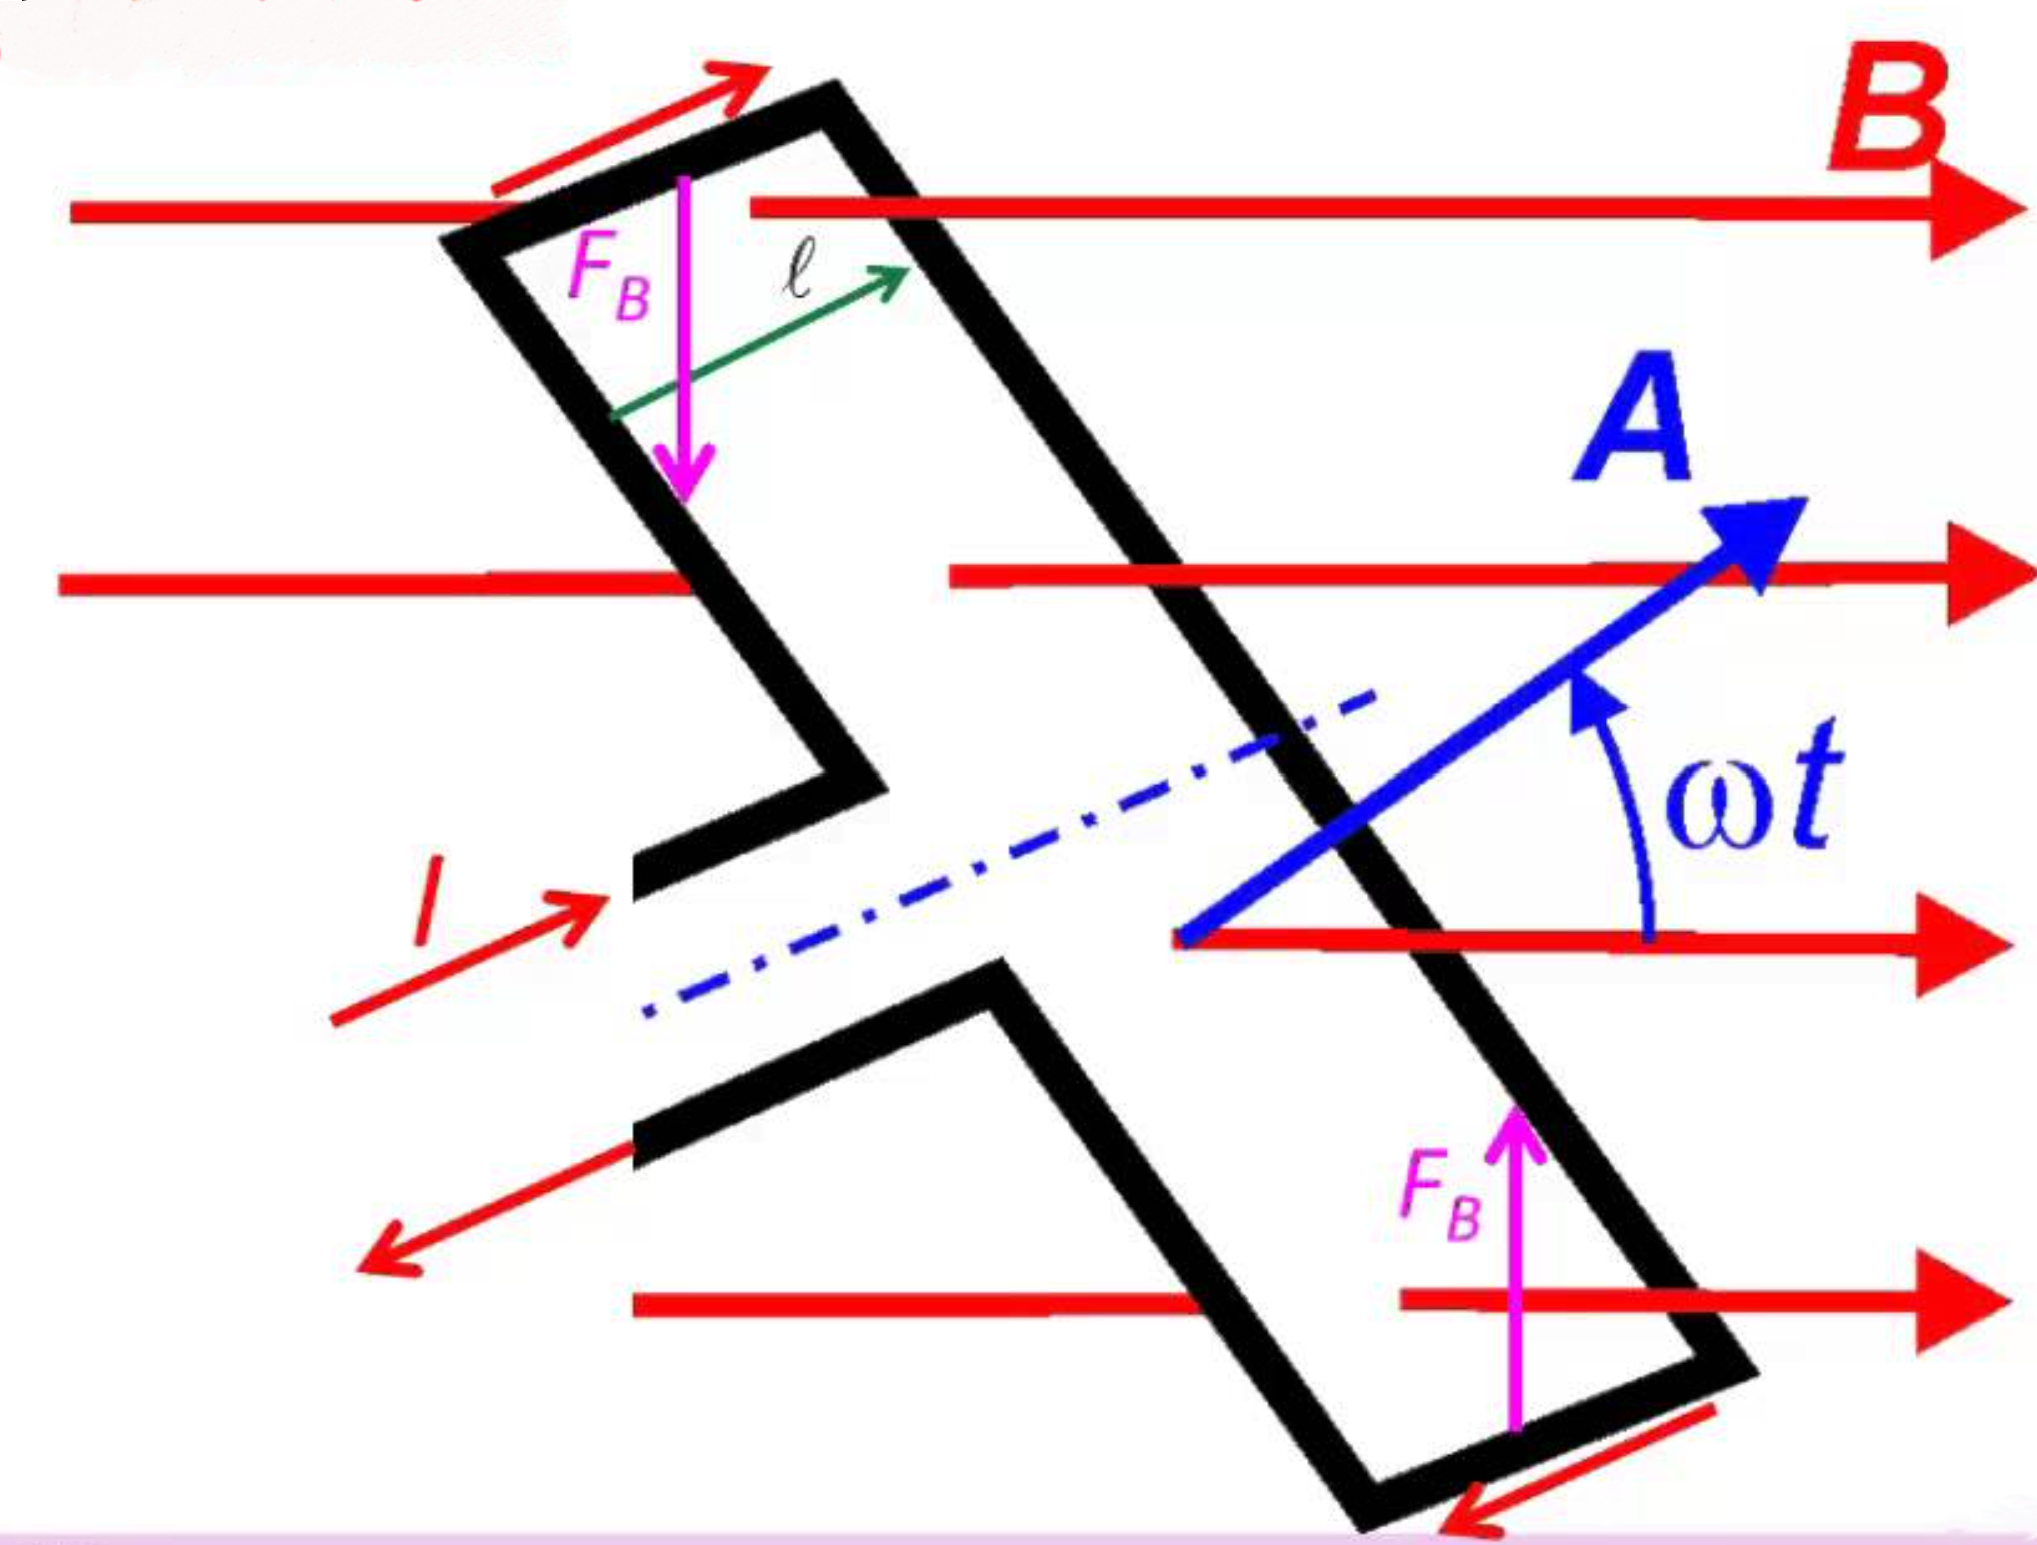
\includegraphics[width = \linewidth]{src/images/leiterschleife.png}
        \end{minipage}

    \subsubsection{Beispiel Transformator}
        \begin{minipage}{0.49\linewidth}
            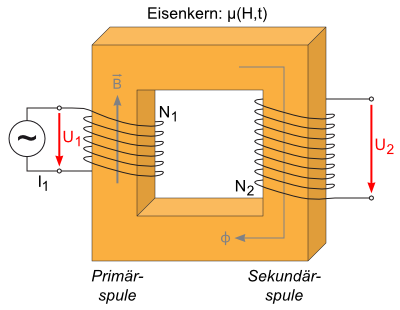
\includegraphics[width = \linewidth]{src/images/transformator.png}
        \end{minipage}
        \begin{minipage}{0.49\linewidth}
            \mathbox{\left| \frac{U_p}{U_s} \right| = \frac{n_p}{n_s}}
            \begin{scriptsize}
                \begin{align*}
                    p &= \text{Primärspule}\\
                    s &= \text{Sekundärspule}\\
                    U &= \text{el. Spannung}\\
                    n &= \text{Windungen}
                \end{align*}
            \end{scriptsize}
        \end{minipage}
%
    \subsubsection{Beispiel parallele stromdurchflossene Drähte}
        \begin{minipage}{0.49\linewidth}
            \includegraphics*[width = 0.8\linewidth]{src/images/magnetische_wirkung_draehte.png}
        \end{minipage}
        \begin{minipage}{0.49\linewidth}
            \begin{itemize}
                \item $\vec{I_1} \uparrow \uparrow \vec{I_2}$: anziehend
                \item $\vec{I_1} \uparrow \downarrow \vec{I_2}$: abstossend
            \end{itemize}
            \mathbox{F_1 = F_2 = \frac{\mu_0}{2 \pi} l \frac{I_1 I_2}{r}}
        \end{minipage}

    \subsubsection{Dynamo}
        Dynamo (Wechselspannung durch sich drehende Schleife in homogenem Magnetfeld):
        \mathbox{U_i = \omega B_0 A_0 sin(\omega t) = U_0 sin(\omega t)}

        \subsubsection{Induzierte Spannung}
        \includegraphics*[width=\linewidth]{src/images/Bsp_induktion_v_aus_abl.png}
\end{document}